\documentclass[]{book}
\usepackage[T1]{fontenc}
\usepackage{lmodern}
\usepackage{amssymb,amsmath}
\usepackage{ifxetex}
\usepackage{fixltx2e} % provides \textsubscript
% use microtype if available
\IfFileExists{microtype.sty}{\usepackage{microtype}}{}
\ifnum 0\ifxetex 1\fi=0 % if pdftex
  \usepackage[utf8]{inputenc}
\else % if xelatex
  \usepackage{fontspec}
  \ifxetex
    \usepackage{xltxtra,xunicode}
  \fi
  \defaultfontfeatures{Mapping=tex-text,Scale=MatchLowercase}
  \newcommand{\euro}{€}
\fi
\usepackage{listings}
\usepackage{ctable}
\usepackage{float} % provides the H option for float placement
\usepackage{graphicx}
% We will generate all images so they have a width \maxwidth. This means
% that they will get their normal width if they fit onto the page, but
% are scaled down if they would overflow the margins.
\makeatletter
\def\maxwidth{\ifdim\Gin@nat@width>\linewidth\linewidth
\else\Gin@nat@width\fi}
\makeatother
\let\Oldincludegraphics\includegraphics
\renewcommand{\includegraphics}[1]{\Oldincludegraphics[width=\maxwidth]{#1}}
\ifxetex
  \usepackage[setpagesize=false, % page size defined by xetex
              unicode=false, % unicode breaks when used with xetex
              xetex]{hyperref}
\else
  \usepackage[unicode=true]{hyperref}
\fi
\hypersetup{breaklinks=true,
            bookmarks=true,
            pdfauthor={},
            pdftitle={TeXstudio : ユーザーマニュアル},
            colorlinks=true,
            urlcolor=blue,
            linkcolor=magenta,
            pdfborder={0 0 0}}
\setlength{\parindent}{0pt}
\setlength{\parskip}{6pt plus 2pt minus 1pt}
\setlength{\emergencystretch}{3em}  % prevent overfull lines
\setcounter{secnumdepth}{0}

\title{TeXstudio : ユーザーマニュアル}
\author{}
\date{}

\begin{document}
\maketitle

\chapter{TeXstudio : ユーザーマニュアル}

\textbf{訳者注:このマニュアルはTeXstudio付属のものを日本語に翻訳したものであり、内容が古いままになっている可能性がある。}

\section{目次:}

\begin{itemize}
\item
  \hyperref[SECTIONNEW]{0. 変更点}

  \begin{itemize}
  \item
    \hyperref[SECTIONNEW262]{Version 2.6.0 -\textgreater{} Version
    2.6.2}
  \item
    \hyperref[SECTIONNEW260]{Version 2.5.2 -\textgreater{} Version
    2.6.0}
  \item
    \hyperref[SECTIONNEW252]{Version 2.5.1 -\textgreater{} Version
    2.5.2}
  \item
    \hyperref[SECTIONNEW251]{Version 2.5 -\textgreater{} Version 2.5.1}
  \item
    \hyperref[SECTIONNEW241]{Version 2.4 -\textgreater{} Version 2.5}
  \item
    \hyperref[SECTIONNEW24]{Version 2.3 -\textgreater{} Version 2.4}
  \item
    \hyperref[SECTIONNEW23]{Version 2.2 -\textgreater{} Version 2.3}
  \item
    \hyperref[SECTIONNEW22]{Version 2.1 -\textgreater{} Version 2.2}
  \item
    \hyperref[SECTIONNEW201]{Version 2.0 -\textgreater{} Version 2.1}
  \item
    \hyperref[SECTIONNEW199a]{Version 1.9.9 -\textgreater{} Version
    1.9.9a}
  \item
    \hyperref[SECTIONNEW20]{Version 1.9.9a -\textgreater{} Version 2.0}
  \item
    \hyperref[SECTIONNEW199]{Version 1.9.3 -\textgreater{} Version
    1.9.9}
  \item
    \hyperref[SECTIONNEW19]{Version 1.8.1 -\textgreater{} Version 1.9}
  \end{itemize}
\item
  \hyperref[SECTION0]{1. TeXstudioの設定}

  \begin{itemize}
  \item
    \hyperref[SECTION01]{1.1 エディターの設定}
  \item
    \hyperref[SECTION02]{1.2 LaTeX関連コマンドの設定}
  \item
    \hyperref[SECTION02a]{1.3 ビルドシステムの設定}
  \item
    \hyperref[SECTION02a1]{1.3.1 ビルドシステムの高度な設定}
  \item
    \hyperref[SECTION030]{1.4 一般的な事項の設定}
  \item
    \hyperref[SECTION03]{1.4.1 スペルチェッカーの設定}
  \item
    \hyperref[SECTION04]{1.4.2 類語辞典の設定}
  \item
    \hyperref[SECTION041]{1.4.3 LaTeX構文チェッカーの設定}
  \item
    \hyperref[SECTION044]{1.4.4 文法チェッカーの設定}
  \item
    \hyperref[SECTION040]{1.5 自動補完の設定}
  \item
    \hyperref[SECTION05]{1.6 ショートカットの設定}
  \item
    \hyperref[SECTION06]{1.7 Latex/Mathメニューの設定}
  \item
    \hyperref[SECTION07]{1.8 カスタムツールバーの設定}
  \item
    \hyperref[SECTION08]{1.9 SVNサポートの設定}
  \end{itemize}
\item
  \hyperref[SECTION1]{2. TeX文書の編集}

  \begin{itemize}
  \item
    \hyperref[SECTION11]{2.1 通常のコマンド}
  \item
    \hyperref[SECTION12]{2.2.1 TeX文書のプリアンブルの設定}
  \item
    \hyperref[SECTION12a]{2.2.2 新規文章作成時のテンプレート使用}
  \item
    \hyperref[SECTION13]{2.3 文書構造}
  \item
    \hyperref[SECTION14]{2.4 文書の閲覧}
  \item
    \hyperref[SECTION15]{2.5 テキストの整形}
  \item
    \hyperref[SECTION16]{2.6 スペース}
  \item
    \hyperref[SECTION17]{2.7 リストの挿入}
  \item
    \hyperref[SECTION18]{2.8 表の挿入}
  \item
    \hyperref[SECTION18a]{2.8.1 表の操作}
  \item
    \hyperref[SECTION19]{2.9 ``tabbing''環境の挿入}
  \item
    \hyperref[SECTION110]{2.10 図の挿入}
  \item
    \hyperref[SECTION110a]{2.10.1 「ウィザード」を用いた図の挿入}
  \item
    \hyperref[SECTION111]{2.11 相互参照及び注釈}
  \item
    \hyperref[SECTION112]{2.12 数式の挿入}
  \item
    \hyperref[SECTION113]{2.13 自動補完}
  \item
    \hyperref[SECTION114]{2.14 類語辞典}
  \item
    \hyperref[SECTION115]{2.15 特殊コマンド}
  \end{itemize}
\item
  \hyperref[SECTION2]{3. 文書のコンパイル}

  \begin{itemize}
  \item
    \hyperref[SECTION22]{3.1 コンパイル}
  \item
    \hyperref[SECTION23]{3.2 ログファイル}
  \end{itemize}
\item
  \hyperref[SECTION3]{4. その他の機能}

  \begin{itemize}
  \item
    \hyperref[SECTION31]{4.1 複数のファイルに分割してある文章について}
  \item
    \hyperref[SECTION32a]{4.2 構文チェック}
  \item
    \hyperref[SECTION32]{4.3 参考文献}
  \item
    \hyperref[SECTION33a]{4.4 SVNサポート}
  \item
    \hyperref[SECTION33]{4.5 私的マクロ}
  \item
    \hyperref[SECTION34]{4.6 Pstricksのサポート}
  \item
    \hyperref[SECTION35]{4.7 Metapostのサポート}
  \item
    \hyperref[SECTION36]{4.8 「HTMLへ変換」コマンド}
  \item
    \hyperref[SECTION37]{4.9 TeXstudioでの「順方向/逆方向 検索」}
  \item
    \hyperref[SECTION\_TEXCOM]{4.10 高度なヘッダの使用法}
  \item
    \hyperref[SECTION38]{4.11 TeXstudioコマンドの概要}
  \item
    \hyperref[SECTION39]{4.12 キーボードショートカット}
  \item
    \hyperref[CWLDESCRIPTION]{4.13 cwl形式の解説}
  \item
    \hyperref[TABLETEMPLATE]{4.14 表テンプレートの使用}
  \end{itemize}
\end{itemize}

\begin{center}\rule{3in}{0.4pt}\end{center}

\chapter{0. 変更点}

\section{Version 2.6.0 -\textgreater{} Version 2.6.2}

\begin{itemize}
\item
  popplerとWindowsでのQt(4.8.5)を更新
\item
  構造ツリービュー:再帰的に構造を閉じる/展開するためのコンテキストメニュー項目を追加
\item
  結合行での厳密な行のワードラップを改良
\item
  「表示 -\textgreater{}
  ビューワーにフォーカスを移動」が別枠ビューワーに対しても機能するように改良
\item
  LanguageToolと辞書の検出が向上
\item
  「列を揃える」がtabu/longtabuに対しても機能するように改良
\item
  多数のバグを修正:編集可能なユーザーテンプレート、右から左向きに読む言語での\}、Macでのpinyin入力メソッドの問題、\ldots{}\ldots{}
\end{itemize}

\section{Version 2.5.2 -\textgreater{} Version 2.6}

\begin{itemize}
\item
  パッケージの解説文書PDFが内部PDFビューワーで表示されるように変更
\item
  モダン形式に対するMacでの完全なretinaサポートを実施
\item
  画面全体でより読みやすくするため、組み込みビューワーを拡大/縮小できるように改良
\item
  最後に開いた(そしてまだ閉じていない)環境をalt+enterで閉じることができるように改良
\item
  「列を揃える」がより多くの環境で機能するように改良
\item
  テンプレートリソースがtemplate\_resources.xmlを通して設定し、utf-8で書かれるように変更
\item
  基本的なPweave強調表示を追加
\item
  \lstinline"% !TeX spellcheck = ..."マジックコメントを追加
\item
  現在の構文強調に依存する新しいマクロトリガーを追加
\item
  右から左方向に読む言語に対する双方向表記サポートの改良
\item
  いくつかの小さな修正
\end{itemize}

\section{Version 2.5.1 -\textgreater{} Version 2.5.2}

\begin{itemize}
\item
  任意の領域を折りたたみ可能としてしるし付けするための\%BEGIN\_FOLD
  \ldots{} \%END\_FOLDコメントを新規追加
\item
  PDFビューワーでCJKとキリル文字の表示のサポートを追加
\item
  タブ幅の最大値を32へ増加
\item
  基本的なインプットメソッドのサポートを修正
\item
  LinuxとMac OS Xでのテンプレートの欠損を修正
\item
  Mac OS Xでメニューバーが消える問題を修正
\item
  すでに開いているファイルとして保存する際にクラッシュする点を修正
\item
  長いステータスメッセージのせいでビューワーのサイズが変化しうる問題を修正
\item
  「次/前の文章」に対するショートカットをCtrl+PgDown/Upに変更
\item
  いくつかの小さな修正
\end{itemize}

\section{Version 2.5 -\textgreater{} Version 2.5.1}

\begin{itemize}
\item
  新しいテンプレートシステム
\item
  折りたたみパネルの改良
\item
  エディターとビューワーでの前方向/後方向マウスボタンのサポートを追加
\item
  インラインプレビューのコンテキストメニューの追加(プレビュー画像のコピー可能に)
\item
  参照/コマンドの概要を完全にするためすべての含まれるファイルの読み込みのオプションを追加
\item
  \textbackslash{}bibliography\{\}コマンドに対する「開く」コンテキストメニュー項目とリンクの重ねあわせの追加
\item
  図の名前の上に来た時に図のプレビューを表示
\item
  いくつかのバグ修正(PDFのスクロール範囲、ユーザーテンプレートパス、OSX関連のバグ、\ldots{}\ldots{})
\end{itemize}

\section{Version 2.4 -\textgreater{} Version 2.5}

\begin{itemize}
\item
  カーソル履歴の追加(後退/前進)
\item
  参照、パッケージ、インクルードされるファイルの名前をCtrl+MouseOver時にリンクになるよう変更
\item
  手書きの数式の挿入機能を追加(Windows 7のみ、TexTablet使用)
\item
  好みの書式を指定するオプションを含む、表コード書式の改良
\item
  LaTeXテンプレートと表テンプレートでのメタデータのサポートを追加
\item
  ランタイムライブラリのバージョンが正しいか確認する機能を追加
\item
  コンテキストメニューをさらに追加(折りたたみパネル、ブックマークパネル)
\item
  より見やすくするためもっと太いカーソルをオプションとして追加
\item
  行操作の追加:上/下へ移動、重複行への操作
\item
  Windowsインストーラー:.texファイルをTXSへ関連付ける選択肢を追加
\item
  いくつかのバグ修正(クラッシュ、コンパイル、焦点移動、\ldots{}\ldots{})
\end{itemize}

\section{Version 2.3 -\textgreater{} Version 2.4}

\begin{itemize}
\item
  いくつかのコマンドを容易に組み合わせることができるビルドシステムに刷新
\item
  多数の新ツールのサポート:xelatex, lualatex, biber, latexmk, texindy
\item
  埋め込みPDFビューワーを追加
\item
  ブックマークマネージャと永続的ブックマークを追加
\item
  LanguageToolを用いたインライン文法チェックを追加
\item
  luaとdtxファイルの構文強調表示を追加
\item
  biblatexサポートを追加
\item
  他のアプリケーションから引用を挿入する引用APIを追加(JabRefプラグインを利用可能)
\item
  表の自動整形
\item
  外観の改良
\item
  アップデートチェッカーを追加
\item
  スクリプトの拡張:GUI/ダイアログの作成、他の文章/プログラム/メニューへの接続、バックグラウンドモードとイベント
\item
  クラッシュからの保護機能を追加
\item
  多数のちょっとした改良
\item
  いくつかのバグ修正
\end{itemize}

\section{Version 2.2 -\textgreater{} Version 2.3}

\begin{itemize}
\item
  \textbackslash{}ref/\textbackslash{}citeの参照を変更可能なコマンドのリストを追加
\item
  検索履歴の記録機能を追加
\item
  文章ごとに異なる辞書を使用する機能のサポートを追加
\item
  無効な括弧を見つける機能を追加
\item
  ほぼ単語レベルでの逆方向PDF検索機能を追加
\item
  図の挿入マクロでのファイル名の補完機能を追加
\item
  BibTeXの自動呼び出し機能を改良
\item
  スクリプトで利用可能な更に多くの手法を追加
\item
  いくつかのバグ修正(特にPDFビューワー/構文チェック/構造ビューでのクラッシュ)と細かい改良
\end{itemize}

\section{Version 2.1 -\textgreater{} Version 2.2}

\begin{itemize}
\item
  プレビューの改良:

  \begin{itemize}
  \item
    PDFビューワーで複数のページを連続して表示可能に改良
  \item
    PDFビューワーを(マルチスレッドで)非停止で機能するように改良
  \item
    プレビューがインクルードされたファイルで機能するように改良
  \end{itemize}
\item
  任意のユーザーマクロを実行できるようにキーを置換
\item
  ダブルクォートの置換を予め定義しておいたリストから容易に選択できるよう改良
\item
  補完で通常のコマンド、最も頻繁に使用されるもの、すべての選択可能なものの区別をするように改良
\item
  プロファイルの保存/読み込みが機能するように改良
\item
  構文強調される環境を増加
\item
  バグ修正と細かい改良
\end{itemize}

\section{Version 2.0 -\textgreater{} Version 2.1}

\begin{itemize}
\item
  オンラインLaTeXの構文チェックの拡張

  \begin{itemize}
  \item
    表中の列数のチェック
  \item
    文章中でどのコマンドが有効か決めるために\textbackslash{}usepackageと\textbackslash{}documentclassを利用するように改良
  \item
    新規コマンドの追加
  \end{itemize}
\item
  TXSが読み込んだ文章の親/子関係を自動検出しそれに応じて振る舞うように変更。従ってマスターモードはもう必要ない。
\item
  プレビューの改良:

  \begin{itemize}
  \item
    PDFビューワーで複数のページを開けるように改良
  \item
    PDFビューワーでのプレゼンテーションモードと複数ビューのサポートを追加
  \item
    PDFビューワーの外観と時計ドックを更新
  \item
    選択部プレビューの高速化とテキスト中表示への対応
  \end{itemize}
\item
  括弧の選択の容易化
\item
  バグ修正と細かい改良
\end{itemize}

\section{Version 1.9.9a -\textgreater{} Version 2.0}

\begin{itemize}
\item
  PDFビューワーと順方向/逆方向検索を結合
\item
  (単純なエラーに対する)オンラインLaTeXの構文チェックを追加
\item
  表の操作をサポート(行、列、あるいは\textbackslash{}hlineの追加/削除)
\item
  挿入された括弧を自動的に閉じるように変更
\item
  厳密な折り返しを伴う行の長さを制限するオプションを追加
\item
  単語の繰り返しを潜在的なスタイルの間違いとしてしるし付けするように改良
\item
  バグ修正と細かい改良
\end{itemize}

\section{Version 1.9.9 -\textgreater{} Version 1.9.9a}

\begin{itemize}
\item
  Macでのいくつかのパフォーマンス問題への取り組み。Macでの長い行を高速化。
\item
  ひとつ以上の重ね書きを同時に表示可能に改良(例:構文強調とスペルチェック)
\item
  補完されたコマンドのコマンド置換を追加
\item
  切り取りバッファを追加。選択されたテキストが補完を通じてコマンドで置換された場合、除去されたテキストが挿入されたコマンドの引数として使用される(適用できる場合)。
\item
  補完でのツールチップで選択された参照の示すラベルの周囲が表示されるように改良
\item
  予め定義しておいたショートカット、メニューの再定義、エディターの設定を含むプロファイルのファイルからの取り込みを追加
\item
  環境名上でテキストカーソルが待機しているときに、その環境名を(\textbackslash{}beginと\textbackslash{}end同時に)変更できるミラーカーソルを生成するように改良
\item
  ALT-delのタイプで単語やコマンド、環境を削除するように改良
\item
  既知のテキストコマンドでのみスペルチェックを行うように変更
\item
  いくつかのダイアログを小さな画面サイズでもよりうまく対処できるように修正
\item
  ユーザーフィードバック後多数のバグを除去
\end{itemize}

\section{0.2 Version 1.9.3 -\textgreater{} Version 1.9.9}

\begin{itemize}
\item
  現在の文書を操作するためのjavaスクリプトがユーザータグで使用可能になる。直接のカーソル処理を通じて操作。さらなる機能が必要な場合、自由に機能要望を上げてよい。
\item
  Macでのいくつかのパフォーマンス問題への取り組み。まだ完全ではないが、Mac上でずっと速く感じるはず。
\item
  式の境界(\$、begin\{equation\}、\ldots{}\ldots{})上にマウスを合わせると数式構造物をプレビューできるように変更
\item
  ツールバーをカスタマイズ可能に変更
\item
  Math/LatexメニューでのLaTeXの式をユーザーの好みのバージョンに変更可能に改良
\item
  開いている文書すべてに対する全検索の改良
\item
  SVNを通じたテキスト文書の透過的なバージョン管理のサポート
\item
  構造ビューとカスタムコマンド補完をタイプした時に更新されるように改良
\item
  構造ビューで付録の一部やインクルードされたファイルの欠如のようなところを色付けするように変更
\item
  マスター文書が定義してある場合、開いてある(!)サブ文章から参照とラベルを対話式のラベルチェックと補完に用いることができるように改良
\item
  ddeコマンドを対応するプログラムが起動していない場合に起動するよう改良
\item
  起動したLaTeXがフリーズした場合に2秒後にエスケープキーを押すことで停止できるよう改良
\item
  折りたたみは今や本当に有益である:不一致な括弧があってももはや折りたたみに支障ないし、折りたたまれたブロックを編集することも可能
\item
  ユーザーフィードバック後多数のバグを除去
\end{itemize}

\section{Version 1.8.1 -\textgreater{} Version 1.9}

TeXstudioは前の月の間にこつこつと拡張されてきた。
次のリストは新しく追加された機能や変更されたもののおそらく不完全な概要である:

\begin{itemize}
\item
  動的な構文強調の最初のステップを実装してきた。
  例えば、\textbackslash{}labelや\textbackslash{}refのようなコマンド中の参照がチェックされ、
  (参照の場合)その参照が存在しない場合や複数回定義されている場合にはしるし付けられる。
\item
  単語補完システムを拡張してきた。
  今や既知のコマンドを相当数に拡張している``kile''の単語リストを使用している。
  bashシェルのように現在の候補リスト中で共通の単語ベースの補完をTabキーで行える。
  更に、以前に使用されたテキスト部分を提示することで通常のテキストをも補完できる。
  この2つのモードはバックスラッシュが開始文字かどうかで区別される。
  そして最後に、補完プロセス時に置換されたユーザー定義の略語を用いて``ユーザータグ''(ユーザー定義のテキストブロック)を挿入できる。
  キーシーケンスを用いてユーザータグを挿入する以前の方法はまだ利用可能である。
  終わりに、ユーザー定義のLaTeXコマンドは自動的にスキャンされ、コマンド補完で使用出来る。
\item
  ウィザードを使う場合は別として、テンプレートを用いて新しく文章を作成できる。
  ユーザーは必要に応じてあとで編集したり削除したりできる自分のテンプレートを追加できる。
\item
  記号パネルが拡張された。``kile''の記号リストでも拡張された。
  また原文そのままのリストから``タグ''を挿入できる。
  そして最後に、列のカウントが利用可能な水平方向のスペースに自動的に適応する。
  不必要な記号リストを隠せることは言うまでもない。
\item
  記号リストセレクタをより空きを増やすためtexmakerのように左端に移動した。
\item
  カーソルを合わせた際のヘルプを実装した。
  カーソルを標準のLaTeXコマンドの上に合わせるとツールチップヘルプが表示される。
  参照の上に合わせた場合、そのラベルを含む対応するテキストメッセージがツールチップとして表示される。
\item
  選択したテキストのプレビューをステータスパネルかツールチップとして表示するようにした。
\item
  望むならステータス/ログ/エラーパネルをタブで使用出来る。
\item
  今やオンラインスペルチェッカーは``aや\textbackslash{}''\{a\}のようなエスケープ文字を正しく扱える。
  また、\textbackslash{}ref\{label\}などといった(いくつかの)LaTeXコマンドオプションのスペルチェックを控える。
\item
  構造ビューのコンテキストメニューで節全体の選択や節のインデントといった有益なオプションを実行できる。
  これは\textbackslash{}sectionを\textbackslash{}subsectionに変更し、それに応じてすべての含まれる見出しも変更することができることを意味している。
\item
  類語辞典を追加した。これで単語の一部でも検索できるようになった。
\item
  確かに多数のバグを潰してきた!
\end{itemize}

\chapter{1. TeXstudioの設定}

TeXstudioを使用する前に、「オプション」メニュー(Mac OS
Xでは「好みの設定」)の「TeXstudioの設定」を通じてエディターとLaTeX関連のコマンドの設定をすべきである。
注意すべきは詳細には2段階あることだ。
より高度なオプションやあまり使用しないオプションは、左下隅の「高度なオプションの表示」にチェックをした場合にのみ表示される。

\section{1.1 エディターの設定}

エンコーディングとしてUTF8を使用したくない場合には、新規ファイルに対する既定のエンコーディングを変えることができる(「TeXstudioの設定」
-\textgreater{} 「エディタ」 -\textgreater{}
「既定のフォントエンコーディング」)。
忘れずに文書中のプリアンブルで同じエンコーディングをセットするように(例:UTF8を使用している場合、\textbackslash{}usepackage{[}utf8{]}\{inputenc\})。\\
TeXstudioはUTF8とlatin1エンコーディングファイルを自動検出できるが、既存の文書で異なるエンコーディングを使用する場合は開く前に設定ダイアログでエンコーディングを指定する必要がある(そして自動検出も無効にする必要がある)。

\begin{itemize}
\item
  「折りたたむ」はエディターのコード折りたたみ機能を有効/無効化する(テキストのセクションを隠す)。
\item
  選択ボックス「字下げモード」では、Enterキーを入力後同じインデントの行にインデントされる行を揃えるか、TeXstudioの自動インデントに任せるかを選択できる。
\end{itemize}

\begin{figure}[htbp]
\centering
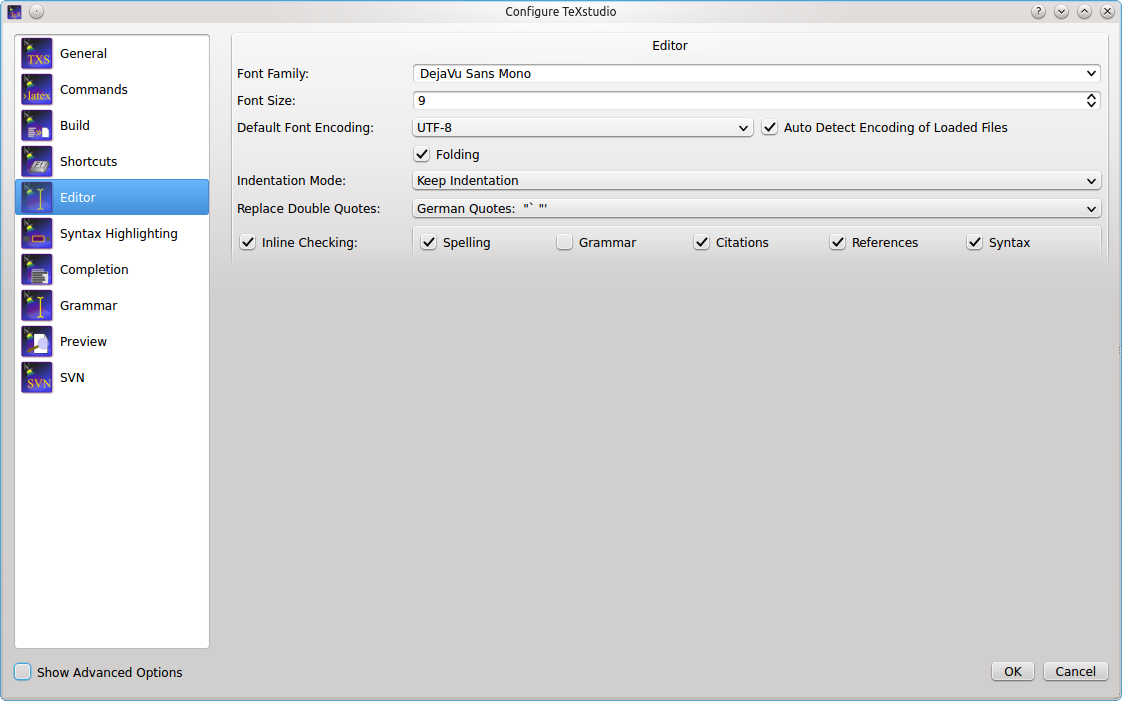
\includegraphics{configure_editor.png}
\caption{エディターの設定}
\end{figure}

\section{1.2 LaTeX関連コマンドの設定}

LaTeX関連コマンドのパスが間違っているとTeXstudioでの文書のコンパイルができない。\\
既定の設定は最近の標準的なLaTeXディストリビューションで機能するが、それらを変更しても良い(「TeXstudioの設定」
-\textgreater{} 「コマンド」)。
コマンドを変更するには、単に対応する行の終わりのボタンをクリックしてファイルブラウザでコマンドを選択すれば良い:
TeXstudioはコマンドの構文に自動的に適応する。\\
\textbf{\%}文字は拡張子なしのファイル名を表し、\textbf{@}文字は現在の行番号に置換される。
更にオプションが必要なら(例:絶対パス)、設定ダイアログの下部の説明を見て?を使用する。\\
\hyperref[SECTION37]{順方向/逆方向検索}の節では一般的なビューワーのコマンド例がいくつか挙げられている。\\
また、右側の「規定値に戻す」ボタンで初期設定にいつでも戻すことができる。

\begin{figure}[htbp]
\centering
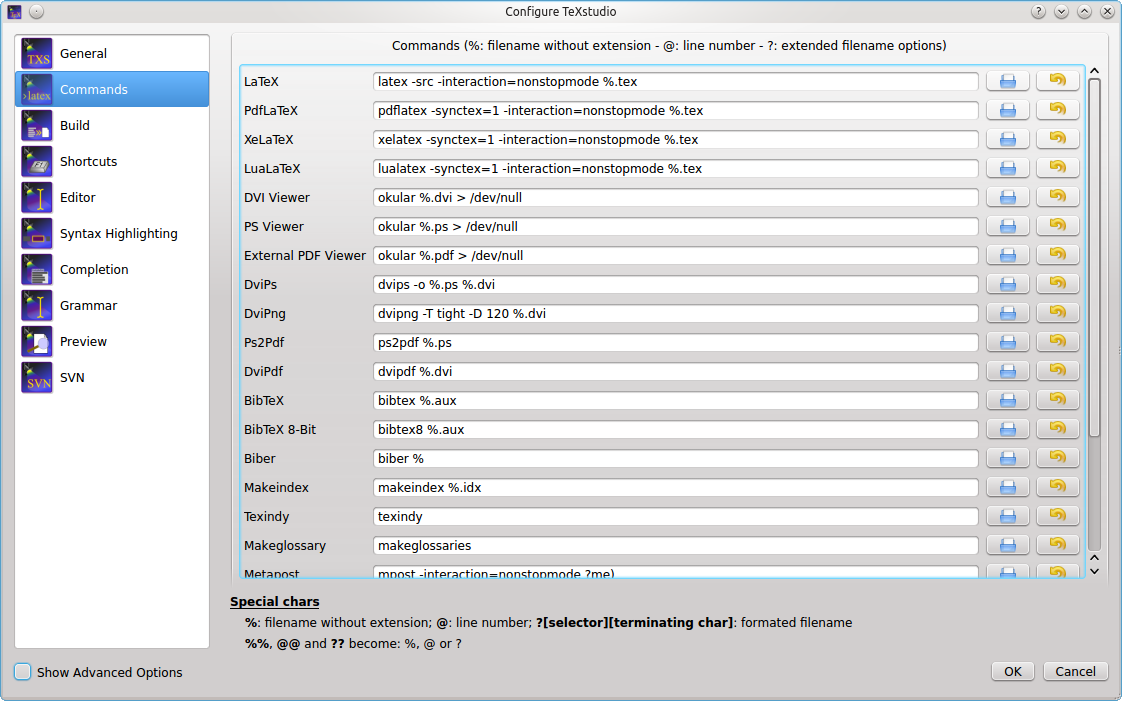
\includegraphics{configure_commands.png}
\caption{コマンドの設定}
\end{figure}

\section{1.3 ビルドシステムの設定}

TeXstudioではLaTeXを変換する一般的なコマンドが提供されている。\\
既定の設定では``pdflatex''と組み込みのPDFビューワーを使用する。
また、別の参考文献変換器と同様に他のコマンドやビューワーを選択することができる。\\
「組み込みPDFビューワー」ではPDF文書を閲覧する際に新しくウィンドウは開かれず、エディターのテキストの隣に直接表示される。\\
有益な別の方法として``latexmk''をコンパイルコマンドとして使用する方法がある(システムにコマンドがインストールされている場合)。
``latexmk''ではbiblatexと索引で依存関係を非常にうまく扱える。\\
更に、高度なオプションでは一般的には必要ないより詳細なカスタマイズを行える。\\

\begin{figure}[htbp]
\centering
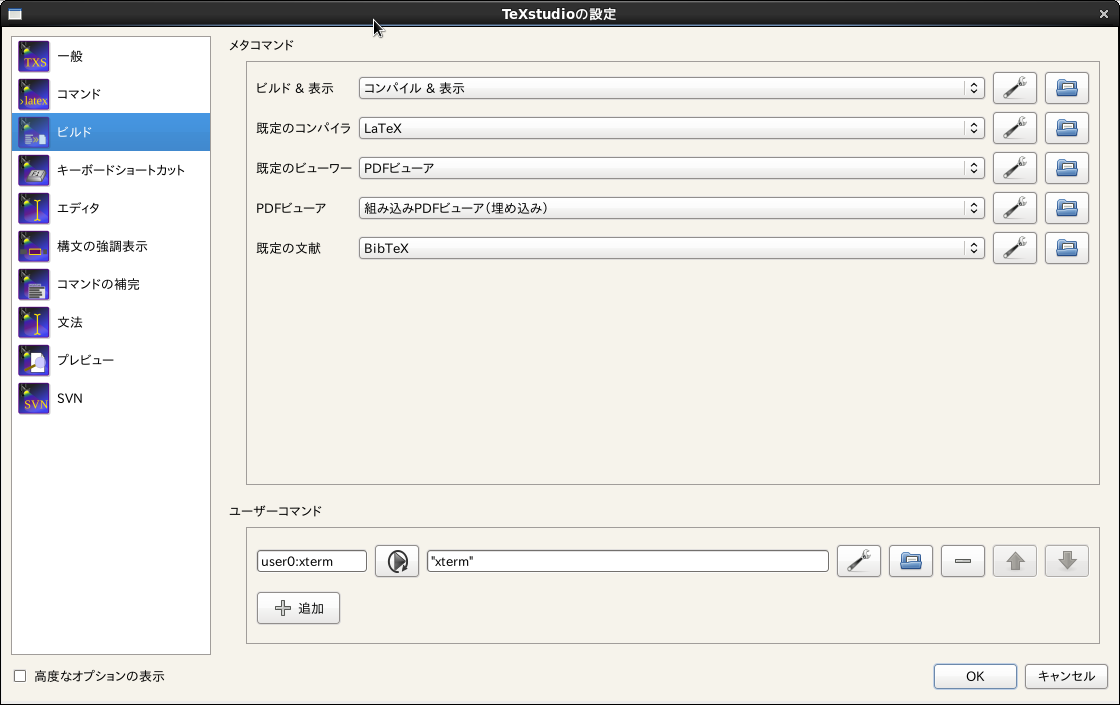
\includegraphics{configure_build.png}
\caption{ビルドシステムの設定}
\end{figure}

ここでユーザーコマンドを「追加」することで定義できる。
各々のユーザーコマンドには``user\%n:''のような名前がつく(``\%n''は数字)。
コロンの後にはツールメニューで表示される名前を記述できる。
ユーザーコマンドはショートカット(alt+shift+F\%n)またはツールメニュー(ツール/ユーザー)のいずれかで実行できる。\\
ユーザーコマンドは既知のコマンドを利用可能なコマンドのリストから選択して組み合わせてもよい。
この場合スパナマークをクリックすると選択可能になる。\\
別な方法としては、ファイルシステムを通じて直接コマンドを選択してもよい。

\begin{figure}[htbp]
\centering
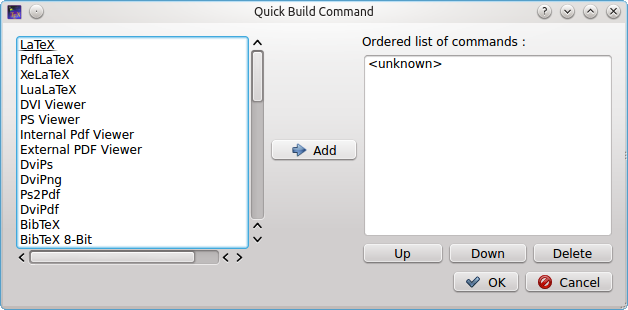
\includegraphics{doc21.png}
\caption{既知のコマンドからのユーザーコマンドの設定}
\end{figure}

\section{1.3.1 ビルドシステムの高度な設定}

高度なオプションを表示するようにしている場合、ビルドシステムをより詳細に設定することができる。

すべてのtxsコマンドは呼び出すべき外部プログラム/LaTeXコマンドと他のtxsコマンドのリストとなっている。
外部プログラムは通常のコマンドラインで呼び出すことができるが、ID``foobar''を持つtxsコマンドはtxs:///foobarで呼び出す。\\
リストのコマンドは単なる区切りである``\textbar{}''で区切られる(``\textbar{}''はあるプログラムからの標準出力を次のプログラムの標準入力へ渡す「パイプ」\emph{ではない})。

これらtxsコマンドにはそれぞれ一意的なIDが付けられ、「通常の」コマンドの、あるいは編集ボックスではユーザーコマンドの名前のツールチップとして表示される。
いくつかの重要なコマンドはよく使用される: txs:///quick
(ビルド&表示、以前のクイックビルド)、 txs:///compile
(既定のコンパイラ)、 txs:///view (既定のビューワー)、 txs:///latex
(LaTeX)、 txs:///pdflatex (pdfLaTeX)、 txs:///view-pdf
(既定のPDFビューワー)、 txs:///view-pdf-external (外部PDFビューワー)。

例えば、典型的なビルド設定ではF1を押してtxs:///quickを呼び出すと、txs:///compileが呼ばれ(まず実際にpdfLaTeXを実行するtxs:///pdflatexが呼ばれる)、そしてtxs:///viewが呼ばれて(txs:///view-pdfが呼ばれ、それによってtxs:///view-pdf-internalが呼ばれる)、PDFが表示される。

コマンド設定ページでコマンドとして定義されたコマンドと、ビルド設定ページでビルドとして定義されたコマンド、ユーザーコマンドとして定義されたコマンドには違いはない。
インターフェースの単純化のためにGUI側で区別しているだけである。\\
これは、前の定義を無視してあらゆるコマンドを望むように変更できる(iniファイルを編集してIDを変えることさえできる)という事でもある。

しかし、常に定義されている三つの内部コマンドがあり、それらは呼び出すことのみ可能で変更はできない:\\\\

\ctable[pos = H, center, botcap]{ll}
{% notes
}
{% rows
\FL
txs:///internal-pdf-viewer & 現在の文書に対して内部ビューワーを開く
\\\noalign{\medskip}
txs:///view-log & 現在の文書に対してログファイルを閲覧する
\\\noalign{\medskip}
txs:///conditionally-recompile-bibliography & bibファイルが変更されているか確認して、変更されている場合txs:///recompile-bibliographyを呼ぶ
\LL
}

内部PDFビューワー(txs:///internal-pdf-viewer)には動作を変更するために次のオプションを使用することもできる:\\\\

\ctable[pos = H, center, botcap]{ll}
{% notes
}
{% rows
\FL
--embedded & ビューワーを埋め込みで開く
\\\noalign{\medskip}
--windowed & ビューワーを別枠で開く(オプションが与えられてない場合の規定値)
\\\noalign{\medskip}
--close-(all\textbar{}windowed\textbar{}embedded) & すべての開いているビューワーを閉じるか、あるいは特定のビューワーだけを閉じる
\\\noalign{\medskip}
--preserve-existing & 既存のビューワーを変更しない(つまり、常に新しいビューワーを開く)
\\\noalign{\medskip}
--preserve-(embedded\textbar{}windowed) & 既存の埋め込み/別枠ビューワーを変更しない
\\\noalign{\medskip}
--preserve-duplicates & 最初に開いたビューワーでのみPDFを開く
\\\noalign{\medskip}
--(no-)auto-close & 対応するtexファイルを閉じた時にビューワーも閉じるかどうか(既定:埋め込みの場合自動的に閉じる)
\\\noalign{\medskip}
--(no-)focus & ビューワーを開いた時にビューワーに焦点を移すかどうか(既定:別枠の場合焦点を移す)
\LL
}

また、呼び出されるサブコマンドの引数を引数変更子または新しい引数の追加で変更することもできる。
これらの変更子は呼び出しリストを通じて渡されるので、直接呼び出されるサブコマンドが別のコマンドの単なるラッパーでも、最終的に呼び出されるプログラムの引数は常に変更される:\\\\

\ctable[pos = H, center, botcap]{ll}
{% notes
}
{% rows
\FL
txs:///foobar --xyz & xyzオプションを追加
\\\noalign{\medskip}
txs:///foobar{[}--xyz=123{]} & xyzオプションの値を123に変更(つまり、foobarで定義されたあらゆるxyzオプションを削除して変更)
\\\noalign{\medskip}
txs:///foobar\{--xyz=123\} & 他の値を持つxyzオプションを無視して、foobarコマンドラインから--xyz=123を削除
\\\noalign{\medskip}
txs:///foobar\{--xyz\} & 値にかかわらず、あらゆる--xyzオプションをfoobarコマンドラインから削除
\\\noalign{\medskip}
txs:///foobar\{\} & 実行可能ファイル名のみ残して、すべてのオプションをfoobarコマンドラインから削除
\LL
}

最後に、iniファイルを変更することでしか変えられない隠しオプションもある:
Tools/Kind/LaTeX、 Tools/Kind/Rerunnable、 Tools/Kind/Pdf、
Tools/Kind/Stdout、 Tools/Kind/Viewer。
これらはそれぞれLaTeXコンパイラ(例えば、後にログを表示する)、再実行可能(警告がある場合にコマンドを繰り返し呼び出す)、PDF生成器(例えば、pdflatex)、標準出力へ出力するコマンド(例えば、bibtex)、そしてビューワー(例えば一度だけ開く)として扱われるコマンドのリストである。

\section{1.4 一般的な事項の設定}

このパネルではいくつかの一般的な外見の設定を行うことができる。

\begin{itemize}
\item
  TeXstudioでは「スタイル」と「配色」を選択できる。
  「配色」のモダンはtexmaker 1.9に似ている。
\item
  記号リストは「タブ形式」で表示されるか(以前の形式、タブ形式が有効な場合)、あるいは記号の空きを多くするため記号リストのそばの小さな記号タブとして表示される。
\item
  ログビューワーもエラー一覧表やログビュー、プレビューワーなどの間をより速く移動できるようにタブ形式で表示される。
\item
  メニューの言語をシステムの設定を無視して直接変更することができる。
\end{itemize}

\begin{figure}[htbp]
\centering
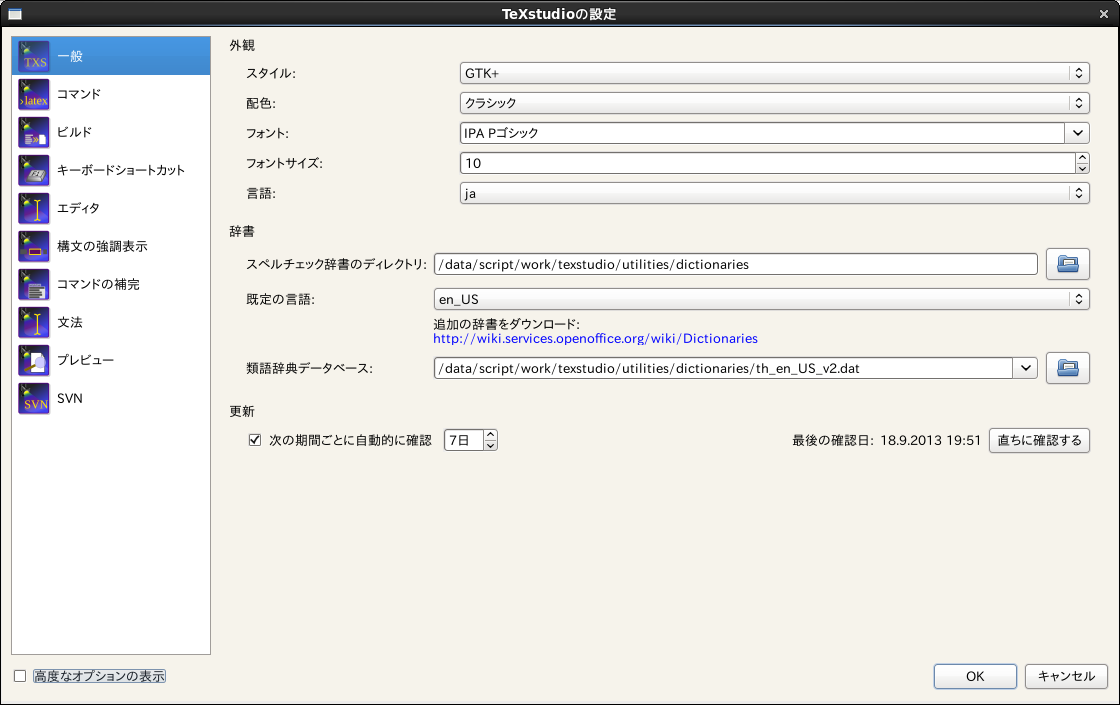
\includegraphics{configure_general.png}
\caption{一般的な設定}
\end{figure}

\section{1.4.1 スペルチェッカーの設定}

TeXstudioでは文字入力中にスペルチェックが行われる。
入力されたテキストがLaTeXコマンドの場合、そのテキストがチェックされるべき自然言語なのか、そのままにしておく単なるコマンドオプションなのかを決めるためにTeXstudioではコマンド補完リストから情報が渡される。
既知のLaTeXコマンドだけがオプションでチェックされる!
既知のコマンドやパッケージについてのさらなる情報については、\hyperref[SECTION040]{補完}の節を参照せよ。\\
スペルチェッカーではOpenOffice.orgの辞書が用いられる。
初期状態ではGPLフランス語、イギリス英語、ドイツ語の辞書がTeXstudioに同梱されている。
他の辞書は\href{http://wiki.services.openoffice.org/wiki/Dictionaries}{http://wiki.services.openoffice.org/wiki/Dictionaries}からダウンロードできる。
すべての辞書はひとつのディレクトリに保存される。\\
簡便のために、TeXstudioではスペルチェッカーの言語を好きに選択できる。
しかし、別の言語で書かれたファイルに対して頻繁に作業する場合規定の振る舞いを上書きしたいと思うかもしれない。
これを行うには二つの方法がある。
一つ目はステータス行の言語メニューを通じてファイルの言語を明示する方法だ。
この設定はファイルを閉じると即座に失われる。
ファイルの言語を永続的に保存するために、TeXstudioは特別な「マジックコメント」\lstinline"% !TeX spellcheck = de_DE"をサポートしている。
このコメントがファイルにある場合、ファイルを開くとその言語に自動的に設定される。

\begin{figure}[htbp]
\centering
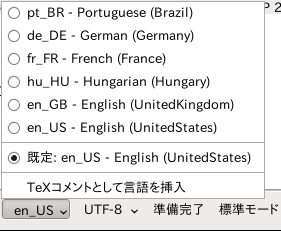
\includegraphics{spellcheck_menu.png}
\caption{スペルチェックメニュー}
\end{figure}

注記:Ctrl+Shift+F7でのスペルチェックはカーソル位置から開始されるのであって、文書の最初からではない。\\\\
もし対話式のスペルチェッカーが有効な場合(既定)、間違って綴られた単語すべてに赤い波下線が引かれる。
その単語で右クリックすると、考えられる訂正語のリストのメニューが表示される。
このコンテキストメニューでは無視するリストにその単語を追加することもできる。
使用している辞書がとても大きい(\textgreater{}
5MB)場合、コンテキストメニューを開いて考えられる候補を表示するのに数秒かかるかもしれない。
もし候補が不必要なら、右クリック中にShiftを押すと待つ必要がなくなる。\\\\
辞書の内部構造が複雑である(例えば、様々な変化形を持つ単語を生成する規則を含む)ので、単純に単語を辞書に追加することはできない。
そのかわり辞書に単語がない場合、その単語を無視するリストに追加してスペルチェッカーが何も言わないようにすることができる。
無視するリストは通常辞書と同じディレクトリに保存される。
それは拡張子が``.ign''のプレーンテキストファイルである。
もし辞書と同じディレクトリに保存できない(例えばアクセス権限がない)場合、そのリストはユーザーの設定ディレクトリに保存される。

\section{1.4.2 類語辞典の設定}

類語辞典ではOpenOffice.org 2.xのデータベースを使用している。
GPLのフランス語、アメリカ英語、ドイツ語のデータベースのみがTeXstudioに同梱されている。\\
ユーザーは次の場所から他のデータベースをダウンロードできる:
\href{http://wiki.services.openoffice.org/wiki/Dictionaries}{http://wiki.services.openoffice.org/wiki/Dictionaries}\\

\section{1.4.3 LaTeX構文チェッカーの設定}

LaTeX構文チェッカーでは、コマンドが正しいかどうか判断するために考えられる完全なコマンドのリストを利用している。
更に、そのコマンドリストには、コマンドがその文脈で有効かどうか、数式モードでのみ有効かあるいは表モードでのみ有効かを決めるための追加情報が部分的に含まれている。\\

\section{1.4.4 文法チェッカーの設定}

文法チェッカーは\href{http://www.languagetool.org/}{LanguageTool}の標準的なhttp
APIに基づいていて、LanguageToolとJavaを別個にインストールする必要がある。

一度LanguageToolをインストールすると、LanguageToolのスタンドアローンアプリケーションを起動し、その後TeXstudioを起動することで文法チェッカーを利用できる。
LanguageToolはアドレスがhttp://localhost:8081/であるローカルで起動するサーバーを作成し、TeXstudioは起動時にそこに自動的に接続される。
接続が確立されたら、すべての入力された段落がLTに送られ、ちょっとした後に考えられる文法上の間違いが強調表示される。

TeXstudioでLanguageToolを自動的に起動させるには、設定ダイアログの文法ページでLT
jarのパスを入力する必要がある。
Javaの実行ファイルが既定のPATHにない場合、そのパスもそこで設定する必要がある。

高度な設定モードでは、あるLTの規則を「特別」として特徴づけすることもできる。
その「特別」な規則に一致したものは異なる/カスタマイズ可能な方法で強調表示される。
これは、例えばLTですべての動詞またはすべての副詞を強調表示する独自の規則を作成することで、文体の解析を行うのに有益である。

LanguageToolとは独立して、TeXstudioでは繰り返しの悪い(不正確な/俗語的な)単語もチェックされる。
繰り返しの確認では、後ろのいくつかの単語を見て、身近なところの短い単語の繰り返しや前方10単語までの長い単語の繰り返しがしるし付けされる。
これらの距離や長さは高度な文法設定のページで変更できる。

\section{1.5 自動補完の設定}

TeXstudioでは、補完用の既知のコマンドの数をかなり増やした、kileの補完単語のリストを採用している。
構文チェックだけでなく補完の有効なコマンドリストを選択するため、TeXstudioでは\textbackslash{}documentclassと\textbackslash{}usepackageが使われていることが認識される。
しかし、TeXstudioでは「TeXstudioの設定」 -\textgreater{}
「コマンドの補完」で追加の単語リストを選択することができる。
単語リストの名前とパッケージ名は対応関係がある。
例えばリストlatex.cwlは標準的なLaTeXコマンドを含んでいる。\\
自動補完に関連して、TeXstudioでは挙動を好みに合わせることができる。
オプションは次のものが利用できる:

\begin{itemize}
\item
  補完の有効化:これは自明である
\item
  大文字と小文字の区別:例えば\textbackslash{}laから\textbackslash{}Largeの補完\ldots{}\ldots{}
\item
  最初の文字で大文字と小文字の区別を行うかどうか
\item
  共通の接頭語の自動補完:リストに一つしか項目がない場合や補完リストのすべての項目の開始文字が共通である場合、Tabキーを押した場合と同様に、共通の文字が直接挿入される。
\item
  非文字キャラクタが押された時に選択したテキストを補完:補完モードではスペースのような非文字キャラクタを押すと、選択した単語を受け入れることになる。
  これによって入力が加速されうる。
\item
  ツールチップヘルプの有効化:補完リストで選択したLaTeXコマンドのヘルプをツールチップとして表示する。
\item
  プレースホルダーの使用:補完されたコマンドに記入すべきオプションがある場合、「プレースホルダー」がその場所に配置される。Ctrl+Right/Ctrl+Leftでそこに移動できる。
\end{itemize}

好みのパッケージが補完(と構文チェック)にない場合、「packagename.cwl」というファイルを設定ディレクトリに配置することで独自のリストを提供できる。
このディレクトリはLinuxでは``\textasciitilde{}/.config/texstudio''、Windowsでは通常``c:\textbackslash{}Documents
and Settings/User/AppData/Roaming/texstudio''である。
基本的にファイルは有効なコマンドのリストを含んでいる。
正確な書式と例の解説は\hyperref[CWLDESCRIPTION]{clw形式の解説}にある。

\begin{figure}[htbp]
\centering
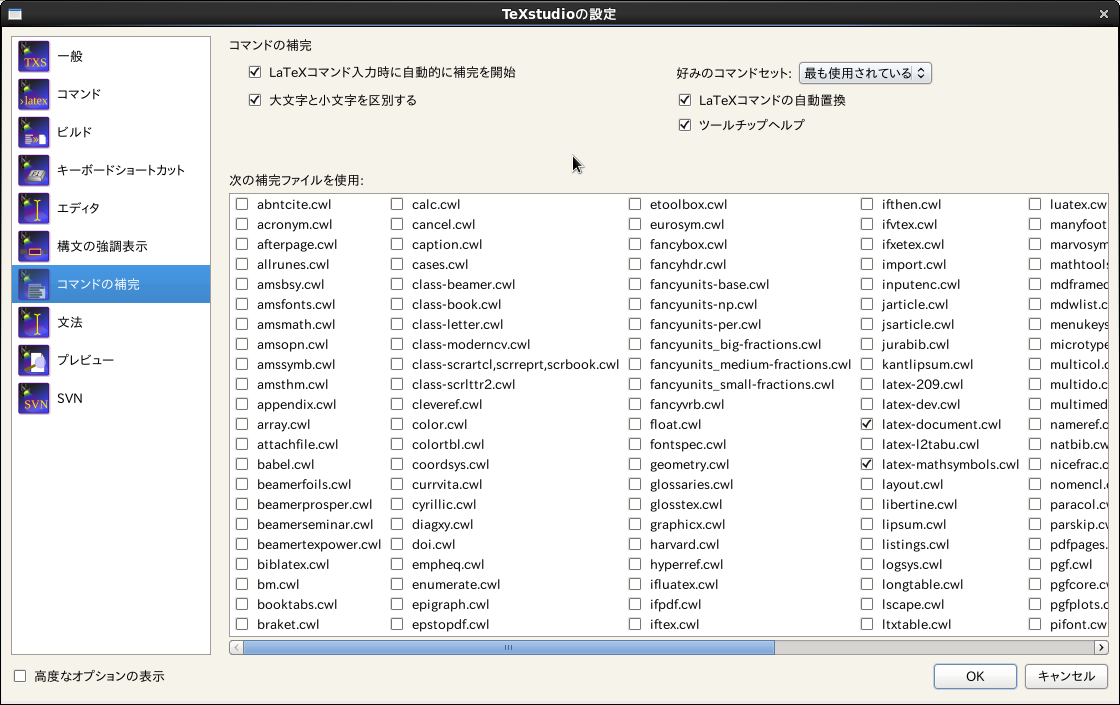
\includegraphics{configure_completion.png}
\caption{補完の設定}
\end{figure}

\section{1.6 ショートカットの設定}

ショートカットは、「現在のショートカット」または「追加のショートカット」の場所でダブルクリックを行うことにより変更できる。
ショートカットは、ドロップダウンリストから選択するか、直接テキストとして入力することができる。
ショートカットを規定値に設定もしくは完全に除去するのであれば、リストの最上部にある「\textless{}default\textgreater{}」または「\textless{}none\textgreater{}」を選択すればよい。

\begin{figure}[htbp]
\centering
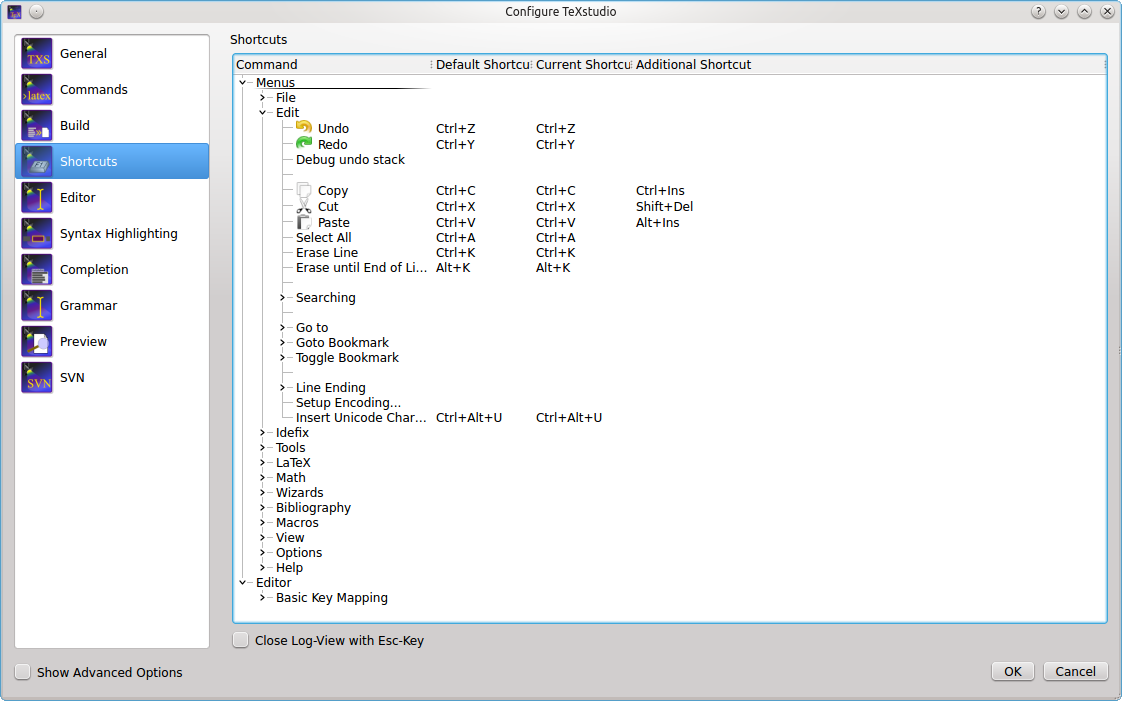
\includegraphics{configure_shortcuts.png}
\caption{ショートカットの設定}
\end{figure}

\section{1.7 Latex/Mathメニューの設定(高度なオプション)}

Math/Latexメニューはユーザーの好みに合わせることができる。
このメニューに対して、項目の名前を変更したり、新規にLaTeXコードを追加したりすることが可能である。
各項目は、ダブルクリックすることで直接編集することができる。

\begin{figure}[htbp]
\centering
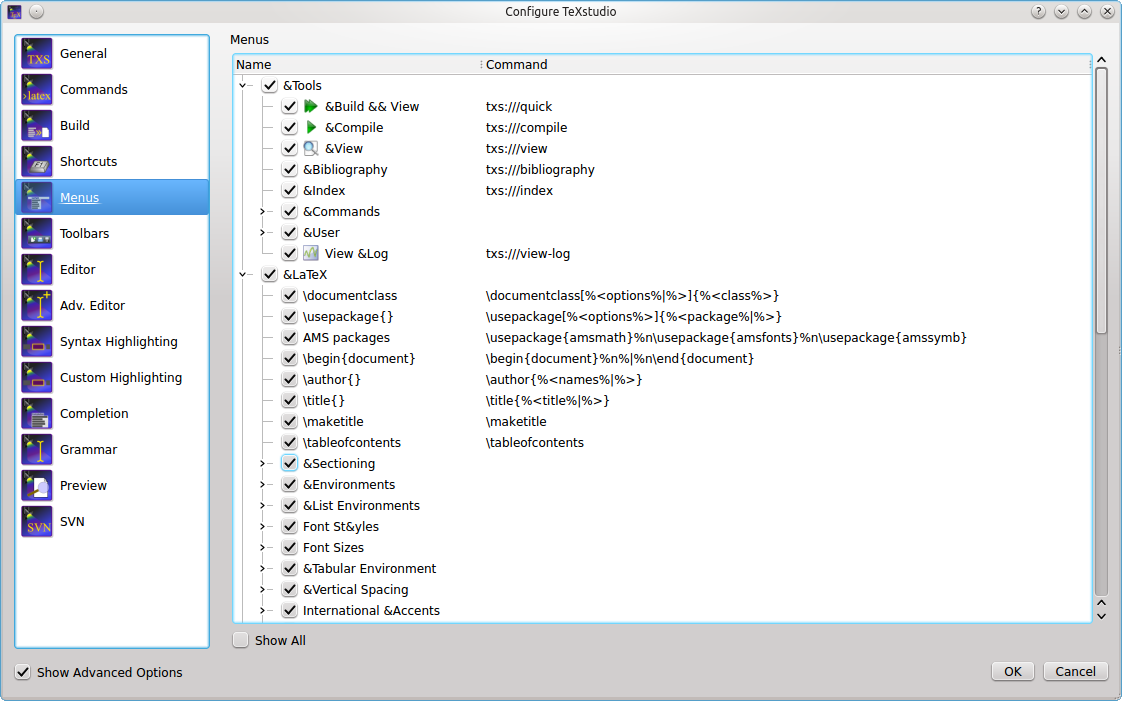
\includegraphics{configure_customizeMenu.png}
\caption{メニューのカスタマイズ}
\end{figure}

\section{1.8 カスタムツールバーの設定(高度なオプション)}

TXSにはカスタムツールバーがひとつ存在する。
このツールバーはLaTeX、Math、ユーザーメニューの要素から成り立っている。
これらの項目の多くにはアイコンがないので、ユーザーが好きなアイコンを読み出すこともできる。
これは、設定ダイアログのカスタムツールバーリストで、項目のコンテキストメニューから「別のアイコンの読み出し」をすることで可能となる。

\begin{figure}[htbp]
\centering
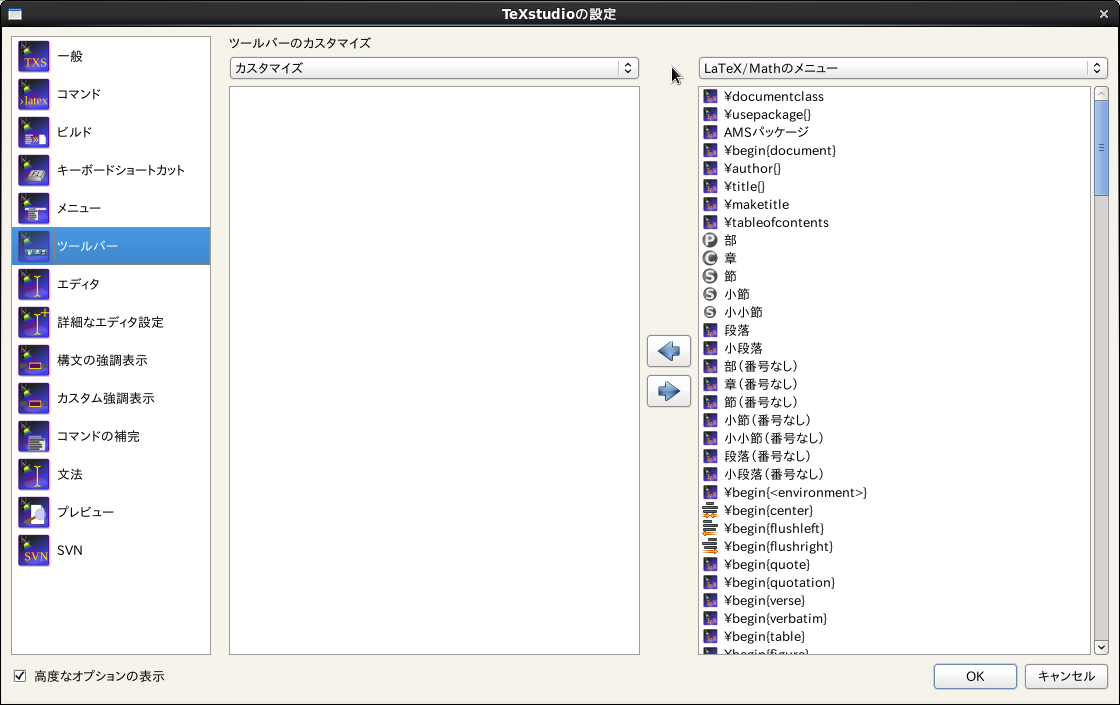
\includegraphics{configure_customToolbar.png}
\caption{ツールバーのカスタマイズ}
\end{figure}

\section{1.9 SVNサポートの設定}

文章のバージョン管理を提供するため、TeXstudioではSVN(Subversion)を使用している。
これを利用するには、SVNコマンドラインツールがインストールされている必要がある。
LinuxとMac
OSXでは通常SVNツールが(パッケージとして)すでに提供されており、Windowsでは「SlikSVN」のインストールが推奨される。

下図のようなSVN設定ページの適切な欄に、「svn」と「svnadmin」のコマンドへの完全なパスが設定されている必要がある。
更に、ユーザーはTeXstudioで提供される自動化の度合いを選択することができる。

「保存後に自動的にチェックインする」を選択すると、TeXstudioが文書を保存するたびにSVNチェックインを行う。
従って文書作成の非常に完全な履歴が残ることとなる。
テキスト文書はディスクの空きスペースに比べて小さいので、SVNのデータベースのサイズは問題にならない。
更に、ディレクトリがすでにSVNの制御下にある場合、(「\ldots{}として保存」で)新たに保存したファイルは自動的にSVNの制御下に追加される。
そうでない場合、TeXstudioは現在のディレクトリ上での「SVNディレクトリの検索深度」のディレクトリ内でSVNの制御下のディレクトリを検索し、サブディレクトリとTeX文書をSVNの制御下に追加する。
適切なディレクトリが見つからない場合、リポジトリが「./repo」というディレクトリに自動的に作成され、文書が追加される。
従って、ユーザーはリポジトリ設定のための必要なコマンドを探す必要はない。
「自動チェックイン」を有効化した場合にのみこの機能は有効化される!

「最後の保存以前に戻すためにSVNリビジョンを用いる」を使うと、TeXstudioはアンドゥを通常のように行うが、内部記憶領域にアンドゥ可能なコマンドがそれ以上ない場合に、文書をSVN履歴での一つ前のバージョンに変更する。
さらなるアンドゥコマンドでより古いリビジョンへ戻すことが可能である一方で、「元に戻す」コマンドでより新しいバージョンへ変更できる。
これは直接メニューコマンドを通してSVNのリビジョンを選択することよりもインタラクティブな手法である(\hyperref[SECTION33a]{4.4章}参照)。

\begin{figure}[htbp]
\centering
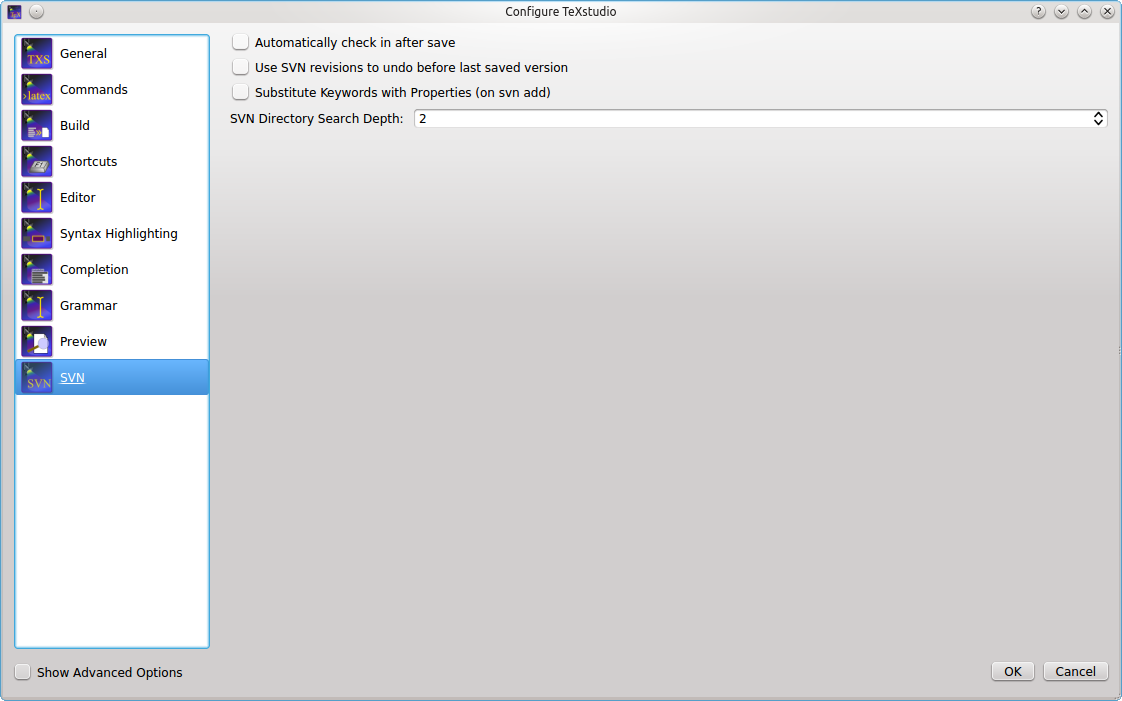
\includegraphics{configure_svn.png}
\caption{SVNの設定}
\end{figure}

\chapter{2. TeX文書の編集}

\section{2.1 通常のコマンド}

標準的なコマンド(切り取り、コピー、検索\ldots{})は「編集」メニューと「編集」ツールバーを通して実行できる。

\begin{figure}[htbp]
\centering
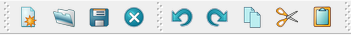
\includegraphics{doc1.png}
\caption{標準的なコマンド}
\end{figure}

\section{2.2.1 TeX文書のプリアンブルの設定}

文書のプリアンブルを定義するには、(「ウィザード」メニューの)「簡単テンプレート」ウィザードが利用できる。

\begin{figure}[htbp]
\centering
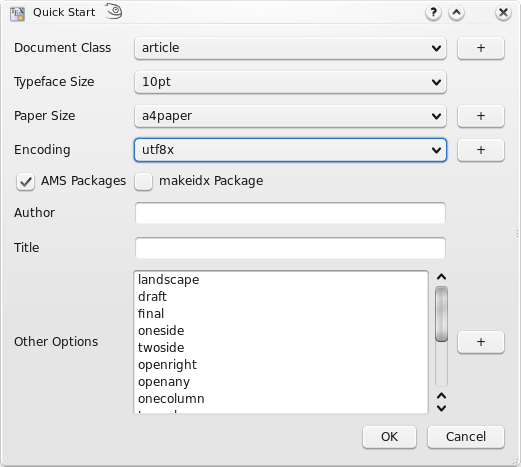
\includegraphics{doc2.png}
\caption{簡単テンプレート}
\end{figure}

このダイアログでは文書の主な仕様(文書クラス、用紙サイズ、エンコーディング、\ldots{})を設定することができる。\\
注意:``+''ボタンをクリックすることで他のオプションを追加することができる。
また、設定全ては記録される。

また、エディターで自分自身のプリアンブルモデルを入力することもできる:「コピー/貼り付け」や「名前をつけて保存」コマンドで、新規文書にそれを利用できる。

\section{2.2.2 新規文書作成時のテンプレート使用}

新規文書に対して、「ファイル/テンプレートから新規作成」コマンドを用いてテンプレートを適応できる。
ダイアログでは利用するテンプレートを選択できる。

\begin{figure}[htbp]
\centering
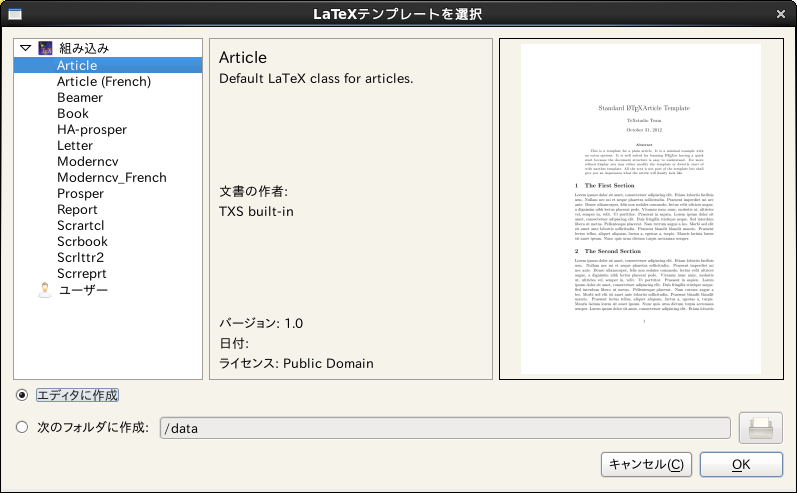
\includegraphics{template.png}
\caption{テンプレート}
\end{figure}

テンプレートから新しいエディター文書を作成するか、テンプレートをファイルとしてディスク上に作成してそれをエディターで開くか選択することができる。
前者のオプションは複数のファイルのテンプレートに対して利用できない。

テンプレートとして利用したい開いている文書に対して、「ファイル/テンプレートを作成」コマンドを用いて新規テンプレートを作成することができる。
このダイアログは現在テンプレートシステムの機能すべてをサポートしてはいないことに注意するように。
特に、プレビュー画像を提供したり、画像つきの複数ファイルテンプレートを作成することはできない。
このようなことは手動で行う必要がある(\hyperref[SECTION12aa]{テンプレートの書式}参照)。

ユーザーが追加したテンプレートは、テンプレート選択ダイアログでコンテキストメニューから編集や削除が可能である。
しかし、組み込みのテンプレートは変更できない。

ユーザーテンプレートは、設定ディレクトリの\lstinline!/templates/user/!サブディレクトリに保存される。

\subsection{2.2.2.1 テンプレートの書式}

最も単純な形式では、テンプレートは.texファイルのみである。
複数ファイルテンプレートはすべてのファイルをzipアーカイブにまとめることで作成することができる。
追加で、同名だが拡張子が``.tex''や``.zip''の代わりに``.json''である別ファイルにメタデータがJSON形式で保存される。
現在次の項目がサポートされている:

\begin{lstlisting}
{
"Name"        : "Book",
"Author"      : "TXS built-in",
"Date"        : "04.01.2013",
"Version"     : "1.1",
"Description" : "Default LaTeX class for books using separate files for each chapter.",
"License"     : "Public Domain",
"FilesToOpen" : "./TeX_files/chapter01.tex;main.tex"
}
\end{lstlisting}

FilesToOpenは複数ファイルの文書に対してのみ影響がある。
テンプレートファイルの隣にプレビュー画像を付け加えてもよい。
ただ、ファイル名は同名で拡張子が``.png''でなければいけない。

\section{2.3 文書構造}

TeXstudioで文書に新しい部分(節、小節、\ldots{}\ldots{})を定義するには、ツールバーのこのコンボボックスを使用すれば良い:

\begin{figure}[htbp]
\centering

\includegraphics{doc3.png}
\caption{区分化}
\end{figure}

これによって、その部分(節、小節、\ldots{}\ldots{})の体裁を定義することができるダイアログがポップアップしてくる。\\
注:「構造ビュー」は自動的に更新される。

\begin{figure}[htbp]
\centering
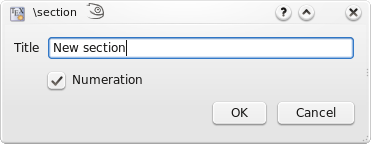
\includegraphics{doc4.png}
\caption{構造ビュー}
\end{figure}

\section{2.4 文書の閲覧}

「構造ビュー」(左側パネル)を用いると、文書のあらゆる部分にすぐに移動できる。
何らかの項目(ラベル、節、\ldots{}\ldots{})をクリックしさえすれば、エディタの対応する場所の先頭へ移動する。
ある行へ移動する仕組みでは、もはや行数を考慮するだけでなく実際のテキスト行をも記憶している。
従って、行を追加や削除しても間違った位置へ移動することはない。

灰色の背景はテキストと構造ビューでの現在のカーソル位置を示している。
緑の背景は付録での節を表している。

\begin{figure}[htbp]
\centering
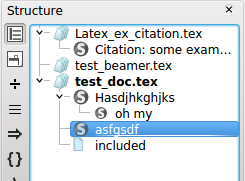
\includegraphics{doc5.png}
\caption{付録}
\end{figure}

「構造ビュー」はタイプしたとおりに自動的に更新される。
また、いつでも(「Idefix」メニューの)「文書構造の更新」コマンドを用いることができる。

ラベル、節、includeやbeamerブロックの他に、\%TODOで始まるコメントもスキャンされて構造ビューに項目として表示される。
これはテキストに一種の永久ブックマークを作成したり、変更が依然として必要な場所を書き留めるために使用することができる。

また構造ビューでは、(小節を含む)節に属するテキストすべてをコピー/切り取りして別の節の前または後ろに貼り付けるコンテキストメニューが利用できる。
更に節のインデント/インデントの解除をすることが可能である。
それは階層構造のレベルを変更することを意味している。
つまり\textbackslash{}sectionが\textbackslash{}subsectionに変更され、全ての小節がそれに応じて扱われる事になる。

それぞれのファイルに対して、移動の高速化のため3つのブックマークが利用できる:ブックマークに追加または削除するには行番号をクリックすれば良い。
すでに3つのブックマークが定義されている場合、新たなブックマークを追加するためそのうち1つを削除しなければならない。
エディタ上でブックマークに対応する行へ移動するには、ステータスバーのブックマークボタンをクリックすれば良い。

\begin{figure}[htbp]
\centering
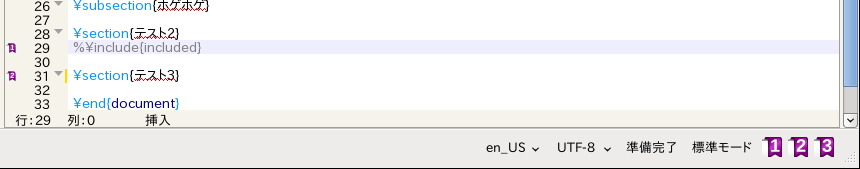
\includegraphics{doc20.png}
\caption{ブックマーク}
\end{figure}

\section{2.5 テキストの整形}

このツールバーでテキストの一部の書式を簡単に設定することができる:

\begin{figure}[htbp]
\centering

\includegraphics{doc6.png}
\caption{書式ツールバー}
\end{figure}

\textbf{追加のオプション:}
選択したテキストを特定の環境で直接囲うこともできる。
例:``Hello''という単語を選択した後「ボールド体」のボタンをクリックすることで、次のコードが入力される:\textbackslash{}textbf\{Hello\}.\\
このオプションは「LaTeX」メニューの``{[}選択{]}''で示されている環境全てに対して利用できる。

\section{2.6 スペース}

通常の「スペース」コマンドは「LaTeX」と「数式」メニューで利用できる。
「強制改行」のLaTeXコマンドを簡単に挿入するには、ツールバーの対応するコマンドを利用できる(ショートカットキー:Ctrl+return)。

\section{2.7 リストの挿入}

通常の箇条書き環境コードは「LaTeX-\textgreater{}箇条書き」メニューから簡単に挿入できる。\\
注:\textbackslash{}itemコマンドのショートカットキーはCtrl+Shift+I.

\section{2.8 表の挿入}

「表作成」ウィザード(「ウィザード」メニュー)で、表環境に対応するLaTeXコードを簡単に挿入することができる:

\begin{figure}[htbp]
\centering
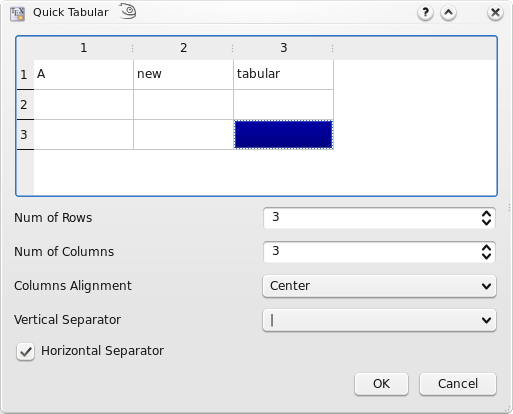
\includegraphics{doc7.png}
\caption{表ウィザード}
\end{figure}

このウィザードで表の主な特徴を設定することができる。\\
注:このダイアログでセルにコードを直接入力することができる。\\
対応するLaTeXコードが自動的にエディタに挿入される。

\section{2.8.1 表の操作}

TeXstudioでは表を簡単に操作できるコマンドが提供されている。
そのコマンドはLaTeX → 表の操作と表ツールバーにある。
表構築のコマンドが複雑になりすぎると予期しない結果となるかもしれないことを認識しておくこと。
次のコマンドが提供されている:

\begin{itemize}
\item
  現在の行の後ろに行を追加
\item
  行を削除:カーソルがある行を削除する
\item
  列の追加:現在のカーソル位置の後ろに列を追加する。
  カーソルが行頭(第一列)にある場合、列は新しい第一列として追加される。
\item
  列の削除:現在の列を削除する
\item
  \textbackslash{}hlineの追加/削除:現在の行以降の全ての行に対して\textbackslash{}hlineを追加/削除する。
  すでに\textbackslash{}hlineのコマンドが存在している場合、二番目のコマンドが置かれることはない。
\item
  列の整列:列区切り記号(\&)を空白記号を挿入することで揃える。
  セルのテキストは表のヘッダーの指定に従って揃えられる。
  これは表のソースを読むのに役立つ。
\item
  テンプレートを用いて表を再構築する。
  これによって文書で同一の表の構築を行うことができる。
  いくつかのテンプレートが予め定義されており、java
  scriptのプログラミングを通して更にテンプレートを追加することができる。
  このコマンドはメニューにしか存在しない。
\end{itemize}

TeXstudioではブロックカーソルも利用できる。
\textless{}Ctrl\textgreater{}+\textless{}Alt\textgreater{}+\textless{}Shift\textgreater{}を押してマウスでカーソルをドラッグすることで利用できる。
ブロックカーソルは通常のカーソルの組のように機能する。
通常と同じくテキストのコピーや貼り付けができる。
また新たなテキストを入力すると、全ての行にそのテキストが追加される。

\begin{figure}[htbp]
\centering
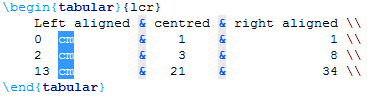
\includegraphics{block_selection.png}
\caption{ブロック選択}
\end{figure}

\section{2.9 ``tabbing''環境の挿入}

``tabbing''コードを挿入するのを容易に行うため、(「ウィザード」メニューの)``Tabbing''ウィザードを利用できる:

\begin{figure}[htbp]
\centering
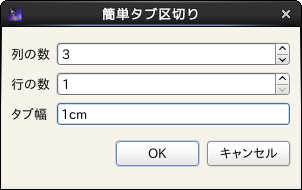
\includegraphics{doc8.png}
\caption{Tabbingウィザード}
\end{figure}

\section{2.10 図の挿入}

文書中に図を挿入するには、「LaTeX」メニューの``\textbackslash{}includegraphics''コマンドを使用すれば良い。
そして画像ファイルを選択するためダイアログの「ブラウザ」ボタンをクリックすれば良い。\\
注:図の挿入前に(「LaTeX - 環境」メニューの)``figure''
LaTeX環境を挿入してもよい。

\begin{figure}[htbp]
\centering
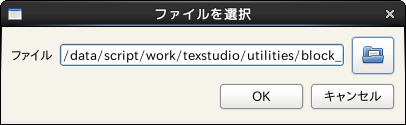
\includegraphics{doc9.png}
\caption{図環境}
\end{figure}

\section{2.10.1 「ウィザード」を用いた図の挿入}

図の適切な挿入は、LaTeX初心者には挑戦であり、熟練者にはほんの僅かのテキストをタイプすることである。
従ってTeXstudioでは文書への画像挿入コードを扱うウィザードを提供している。
「画像オプション」では\lstinline!\includegraphics[options]{file}!のオプションパラメータを定義する。
最も使用される幅/高さの属性は容易に設定できる一方で、ユーザー定義の設定で完全に制御することもできる。\\
画像をテキスト中のまさにその位置に配置する必要がない場合、画像を\lstinline!figure!環境内に置くべきだ。
そしたらLaTeXの方でページ上の最適な位置を決定してくれる。\\
「既定として保存」ボタンを押すことで、現在の設定(ファイル、図見出し、ラベルを除く)が保存される。
そしてウィザードを開いた際その設定を既定として使用することができるようになる。\\
画像ファイルを文書にドラッグ&ドロップしたり、エクスプローラーでコピーしてTeXstudioで貼り付けたりした時にも、画像挿入ウィザードが起動する。
これによって、調整可能な既定パラメータを伴って新しい画像を非常に素早く挿入できる。
更に図のコード上にカーソルがあるときに画像挿入ウィザードを開始すると、既存の図の設定をそのウィザードで操作することができる。

\begin{figure}[htbp]
\centering
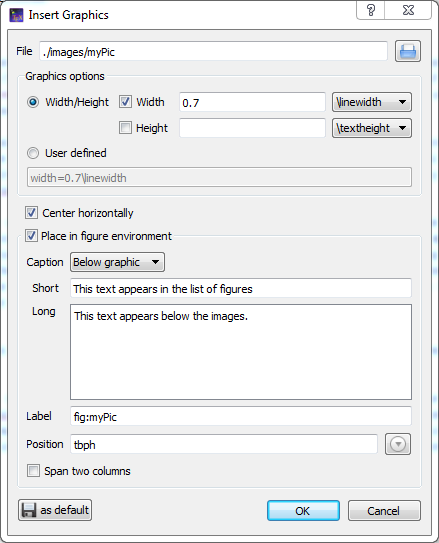
\includegraphics{wizard_figure.png}
\caption{図ウィザード}
\end{figure}

\section{2.11 相互参照及び注釈}

ツールバーのこのツールボックスでラベルや引用、参照、脚注などのコードをすぐに挿入できる。\\
注:文書中で用いられているラベルは「構造ビュー」に表示される。

\begin{figure}[htbp]
\centering
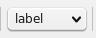
\includegraphics{doc10.png}
\caption{構造ビューのラベル}
\end{figure}

\textbf{追加のオプション:}\textbackslash{}refコマンドに対しては、ダイアログボックスで直接ラベルを選択することができる。

\section{2.12 数式の挿入}

ツールバーの「インライン数式」ボタン(ショートカット:Ctrl+Shift+M)または「数式」メニューで、「インライン数式」環境内の状態へと切り替えることができる。
「ディスプレイ数式」環境のショートカットキーは次である:Alt+Shift+M。\\
「数式」ツールバーで\textbackslash{}leftや\textbackslash{}rightタグのような最も使用される数学的な形(frac,
sqrt\ldots{})を挿入できる。

\begin{figure}[htbp]
\centering
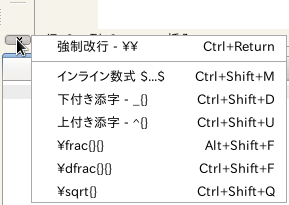
\includegraphics{doc11.png}
\caption{数式ツールバー}
\end{figure}

また、「文書の構造」ビューの「記号パネル」を用いて、400種類の数学記号のコードを挿入することができる。

\begin{figure}[htbp]
\centering
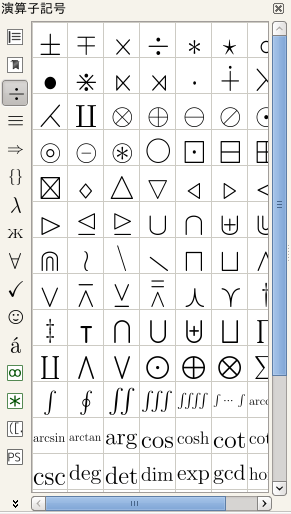
\includegraphics{doc12.png}
\caption{数学記号パネル}
\end{figure}

「数式」メニューを通して数学的テキストの書式を決めることもできる。\\
``array''環境に対しては、(「表」ウィザードのように)「ウィザード」メニューからウィザードが利用できる。
このウィザードでは、使用する環境(array, matrix,
pmatrixなど)を選択することができる。 更にセルを直接埋めることもできる。

\begin{figure}[htbp]
\centering
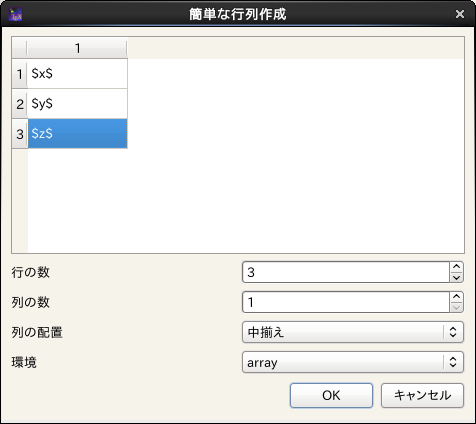
\includegraphics{doc13.png}
\caption{行列ウィザード}
\end{figure}

\section{2.13 自動補完}

``\textbackslash{}''に続いて文字を打つと常に、考えられるLaTeXタグのリストが表示され、正しいものを選択することができる。
追加の文字を打った場合、LaTeXタグリストはフィルター処理されて、すでに書かれたテキストで始まるタグのみが表示される。
タグリストが同じ文字の組み合わせで始まる単語だけを含む場合、Tabキーを押して全てに共通する文字を補完することができる。
もしタグリストに一つしか要素がない場合、EnterキーのようにTabキーでこれを選択して補完することができる。
この振る舞いはbashシェルでのtab補完に似ている。
また、望むときにCtrl+Spaceを押してこのタグリストを開くことも可能である。\\
タグに異なるオプションがある場合、短い説明的なテキストが挿入され、それぞれのオプションの意味を教える。
更に、Ctrl+LeftとCtrl+Rightを押してあらゆる位置を選択することができる。\\
また通常のテキストも単語をタイプし始めてCtrl+Spaceを押すことで補完を行うことができる。
現在の文書の適切な単語全てが考えられる候補として用いられる。\\
環境を挿入するつもりであれば、環境名の最初をタイプしてCtrl+Alt+Spaceを押すことで、適切な環境の候補が表示されて\textbackslash{}begin\{env\}..\textbackslash{}end\{env\}で補完挿入される。\\
そして最後に、ユーザータグを補完で使用することもできる略語へ割り当てることが可能である。
略語の最初の部分をタイプしてCtrl+Spaceで補完を開始するだけでよい。
そうした略語は、特に``略語(テンプレート)''でしるし付けされて補完リストに表示される。\\
もし新たなコマンドを補完することでとあるコマンドを変える場合、コマンド名のみが取り替えられる。
同じことが環境に対しても当てはまり、\textbackslash{}begin- \&
\textbackslash{}end-コマンド内の環境名が変化する。

\section{2.14 類語辞典}

TeXstudioは単純な類語辞典を統合している。 これにはOpenOffice
2.xのデータベースを使用している。
単語上にカーソルを置いて類語辞典をアクティブにする(Ctrl+Shift+F8またはツール/類語辞典)ことで、この単語に対する類義語を見つけようとする。
類語辞典を初めて起動する場合には、データベースの読み込みが生じて少し時間がかかりうるので我慢すること。

\begin{figure}[htbp]
\centering
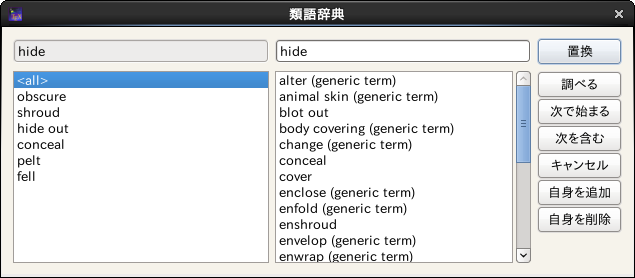
\includegraphics{thesaurus.png}
\caption{類語辞典}
\end{figure}

左側の最初の行は類義語を探索する対象単語を含む。
その下のリストは単語の種類のリストである。
それらのいずれかを選択して候補の数を減らすことができる。
右側の欄は提案された類義語のリストを含む。
このリストから選択した単語が、そのテキストの代わりに対する提案として右側の最初の行に表示される。
この単語は手動で変更できる。
その単語は、それ「で始まる」またはそれ「を含む」単語や類義語に対するさらなる調査にも用いられる。
「調べる」でその単語の類義語を探すために直接利用することもできる。

\section{2.15 特殊コマンド}

\subsection{単語/コマンド/環境の削除}

Alt+Delのショートカットでカーソル位置の単語が削除される。
それがコマンドならば、そのコマンドが開き括弧と閉括弧を含んで削除される。
例:``\textbackslash{}textbf\{text\}''は``text''が残ることになる。
もしも環境だった場合、取り囲むbegin/endが削除される。

\subsection{環境名の付け替え}

カーソルが環境名もしくは対応するbegin-/end-コマンド上にある場合、少ししてミラーカーソルがアクティブになる。
これでbegin-\&end-コマンドの環境名を同時に変更することができる。
もし``\textbackslash{}begin\{tabular\}\ldots{}\textbackslash{}end\{tabular\}''構文を``\textbackslash{}begin\{tabularx\}\ldots{}\textbackslash{}end\{tabularx\}''へ変更したい場合、テキストカーソルを``tabular''の上に置き「環境名の付け替え」を実行して少し待てばよい。
すると、ミラーカーソルが現れて``tabular''を``tabularx''に変更できるようになる。

\subsection{バッファの切り取り}

何かを選択してコマンドを入力し始めて補完を行う場合、選択したものが最初の引数として配置される。
例:``text''があり、それを選択して``\textbackslash{}textbf''を補完入力する。
すると結果として得られるテキストは``\textbackslash{}textbf\{text\}''となる。

\chapter{3. 文書のコンパイル}

\section{3.1 コンパイル}

文書をコンパイルする最も簡単な方法は、「コンパイル」コマンドまたは「ビルド&表示」コマンド(「コンパイル」ボタン
- ショートカット:F6、「ビルド&表示」ボタン -
ショートカット:F1)を使用することである。
「TeXstudioの設定」ダイアログを通して既定のコマンドを選択することができる。\\
(また、「ツール」メニューで各々のコマンドを一つ一つ起動することも可能である。)\\
注:「ツールメニュー」の「補助ファイルの削除」でLaTeXのコンパイル時に生成されるファイル(dvi,
toc, aux\ldots{})を削除することができる(ps&pdfファイルを除く)。\\

\begin{figure}[htbp]
\centering

\includegraphics{compile_toolbar.png}
\caption{コンパイルツールバー}
\end{figure}

\textbf{注意:すべてのファイルには拡張子がなければならず、「タイトルなし」ファイルや名前に空白のあるファイルはコンパイルできない。}.

\section{3.2 ログファイル}

「ビルド」コマンドで、ログファイルが「メッセージ/ログファイル」パネルに自動的に表示される。
もしコンパイル時にエラーが生じれば「エラー」パネルにそのエラーが表示される。
「エラー」パネル上の「行」列の数字をクリックすれば、エディタ上で対応する行にカーソルが移動してそのエラーが「ログファイル」パネル上でも表示される。

\begin{figure}[htbp]
\centering
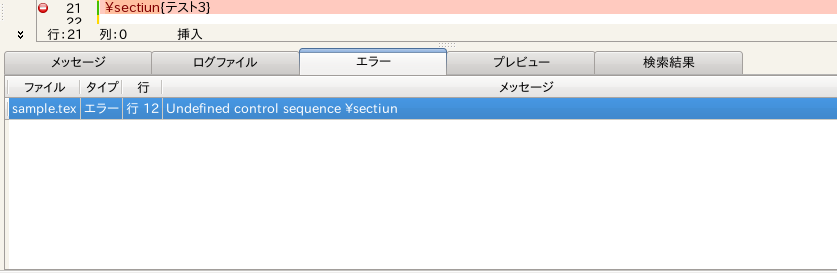
\includegraphics{doc15.png}
\caption{ログファイル}
\end{figure}

「次のエラー」と「前のエラー」コマンドでコンパイル中に検出されたエラーの間を移動できる。

エラーや警告、良くないボックスのある行は背景がそれぞれ赤、黄色、青で強調表示される。
また、Ctrl+Up/Downでそれらの間を移動できる(エラーのみに対してはCtrl+Shift、警告のみに対してはCtrl+Alt、良くないボックスのみに対してはAlt+Shiftを用いる)。\\
更に、それらの行へ移動するとツールチップで間違いのさらなる詳細が表示される(行番号の左側の印にマウスを合わせた場合にも表示される)。

\chapter{4. その他の機能}

\section{4.1 複数のファイルに分割してある文章について}

TeXstudioでは、複数ファイルに分割された文書を扱うことができる。\\
TeXファイルを文書に含めるためには、「LaTeX」メニューの「\textbackslash{}include\{file\}」または「\textbackslash{}input\{file\}」コマンドを使用すれば良い。
そのファイルは「構造ビュー」に表示されることになる。
そのファイル名をクリックすることで、TeXstudioでそのファイルを開くことができる。

TeXstudioは今や読み込んだ文書の親/子関係を理解する(1レベルのみ!)。
従って「マスター文書モード」でのように、子の文書について作業している間コンパイルを開始すると親文書のみがコンパイルされる。
また、対応する全ての文書内のラベルとユーザーコマンドが認識される。

更に、「オプション」メニューで「マスターファイル」を定義することもできる。
「子」文書に対して作業している時でさえ、「ツール」メニューのコマンド全てはマスターファイルに対してのみ適用される(「マスター」ファイルを閉じることすら可能である)。\\
マスターファイルが設定されている場合、開いてある文書で定義されているラベルとユーザーコマンドは開いてある文書全てで補完候補として利用できる。
従って、別のサブ文書で定義されているラベルへの参照をその文書をTeXstudioで開いている限り簡単に挿入できる。\\
注:「オプション」メニューで「マスター」モードを解除できる。

\section{4.2 構文チェック}

LaTeX構文チェッカーは、コマンドが正しいかどうか決めるため考えられる補完コマンドのリストを採用している。
どの文脈でコマンドが有効であるか、例えばコマンドが数式モードでのみまたは表モードでのみ有効なのかどうかを決めるため、補完リストは部分的に追加情報を含んでいる。\\
更に表の正確さはより詳細に確認される。
列の数が続く行で解析・確認される。
もしある行で列の数が多かったり少なかったりすると、警告印が表示される。

\section{4.3 参考文献}

``bib''ファイルに対して、「文献」メニューで文書の標準型に対応する項目を直接挿入できる。\\
注:「文献」メニューの「削除」コマンドでオプション項目が自動的に削除される。

\begin{figure}[htbp]
\centering
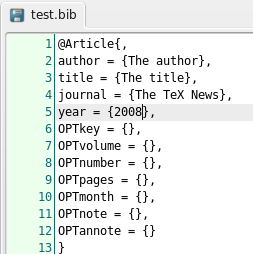
\includegraphics{doc16.png}
\caption{参考文献メニュー}
\end{figure}

\section{4.4 SVNサポート}

第1.8節ですでに述べたサポートされているsvn機能とは別に、TeXstudioはさらに2つのコマンドをサポートしている。

「ファイル/SVN/チェックイン」で、svn履歴に保存されるチェックインメッセージを求める入力ダイアログとともに明示的に保存、チェックインが行われる。

「ファイル/SVN/古いリビジョンを表示」で、全ての利用可能なリビジョンを表示するダイアログが表示される。
古いリビジョンを選択することで、その古いリビジョンへ現在の文書が即座に変更される。
また、古い部分をコピーして最新のバージョンへ戻ることで、その部分を文書の最新バージョンにすることができる。
もしその文書を直接編集し始めると、ダイアログは閉じて現在のテキストが未保存だが新しい最新バージョンとなる。

\section{4.5 私的マクロ}

TeXstudioでは自分のマクロを挿入できる(ショートカット:Shift+F1\ldots{}Shift+F10)。
これらのマクロは「マクロ - マクロを編集」メニューで定義できる。
マクロはTXSに直接配置される単純なテキストからなる。
また、それはbegin/endで自動的に展開される「環境」でも、java
scriptでも良い。 必要な機能はチェックボックスで選択することができる。\\
「略語」はLaTeX補完に対する擬似コマンドである。
擬似コマンドが補完されると代わりにそのマクロが挿入される。
擬似コマンドはバックスラッシュ(``\textbackslash{}'')で始まる必要があることに注意すること。\\
「トリガー」はマクロを含むものを自動実行する正規表現である:
最後に入力された文字がこの表現に一致すると、それは削除されてマクロが挿入/実行される(詳細は\hyperref[sectionTriggers]{下}を見ること)。

\begin{figure}[htbp]
\centering
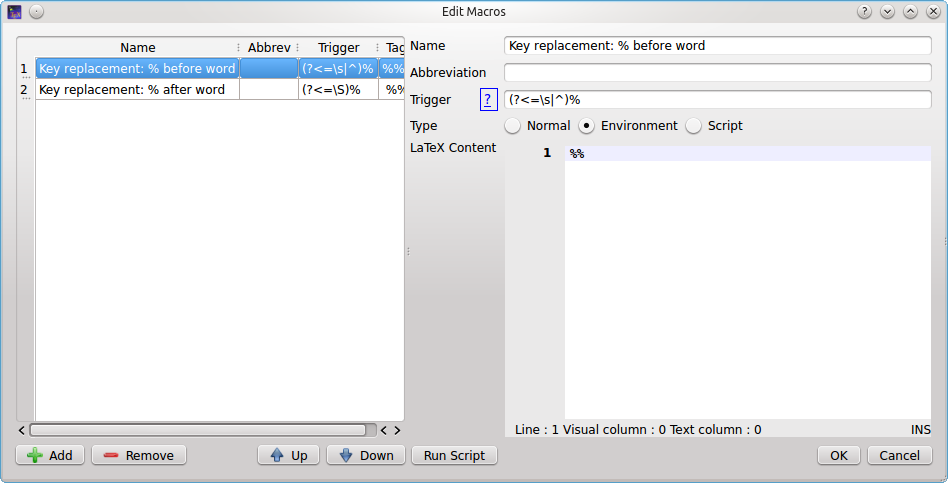
\includegraphics{doc17.png}
\caption{マクロの編集}
\end{figure}

\subsection{4.5.1 テキストマクロ}

通常のテキストとは別に、いくつかの特別なコードが認識されて挿入時に置換される。\\
もしどこかに\%\textbar{}を書いた場合、カーソルは挿入されたテキストのその場所に配置される(2番めの\%\textbar{}はそれらの間全ての選択になる)。\\
\%\textless{}something\%\textgreater{}を書くと、Ctrl+Left/Rightで選択できる説明的テキストとしてしるし付けされる。\\
オプション\%(\emph{filefilter}\%)はファイルダイアログで尋ねられるファイル名で置換される。
ファイルフィルターは標準的なQtファイルフィルター形式である。\\
例:``Images (*.png *.xpm *.jpg);;Text files (*.txt);;XML files
(*.xml)''。
\href{http://qt-project.org/doc/qt-4.8/qfiledialog.html\#getOpenFileName}{Qt-Doc}も参照すること。

\subsection{4.5.2 環境マクロ}

テキストは環境名として用いられる。
従って``\%environment''は次のように挿入される:\\
\textbackslash{}begin\{environment\}\\ \\
\textbackslash{}end\{environment\}\\ \\
注:TeXstudioでは、挿入時に配置されないものの環境名が``\%''で始まる必要がある。

\subsection{4.5.3 Javascriptマクロ}

コード片を用いる代わりに、javascriptを使用することもできる。
そのためには最初の行に``\%SCRIPT''を置けばよい。
続くコードはjavascriptとして解釈される。
言語は\href{http://www.ecmascript.org/index.php}{ECMAScript}に基づく。
文書にアクセスするために次のオブジェクトが導入されている:

\begin{itemize}
\item
  ``editor''で検索/保存/読み込みといった最上位の操作を現在の文書で行うことができる。
\item
  ``cursor''で移動、テキストの挿入や削除といったカーソル操作にアクセスすることができる。
\item
  ``fileChooser''で非常に単純なファイル選択ダイアログにアクセスすることができる。
\item
  ``app''でクリップボードやメニューといったアプリケーションの幅広いものへアクセスすることができる。
\end{itemize}

次の表は考えられるコマンドの概要である。

コマンド

説明

グローバルスコープ

alert(str), information(str), warning(str)またはcritical(str)

文字列strをあるアイコンとともにメッセージボックスに表示

confirm(str)またはconfirmWarning(str)

文字列strをはい/いいえ(yes/no)の質問としてメッセージボックスに表示

debug(str)

文字列strを標準出力stdoutに表示

writeFile(name, value)

ファイルnameに値valueを書き込む(書き込み権限を要求)

readFile(name)

ファイルname全体を読み込む(読み込み権限を要求)

system(cmd)

コマンドcmdを呼び出し、次のメソッドをもつProcessXオブジェクトを返す:

\begin{itemize}
\item
  waitForFinished: プロセスが終了するまで待つ
\item
  readAllStandardOutputStr: 標準出力stdoutを返す
\item
  readAllStandardErrorStr: 標準エラー出力stderrを返す
\item
  exitCode: 終了コード
\item
  exitStatus: Qt終了ステータス
\item
  terminateまたはkill: プロセスを停止する
\end{itemize}

setGlobal(name, value)

一時的なグローバル変数を設定する

getGlobal(name)

グローバル変数を読み込む

hasGlobal(name)

グローバル変数の存在を確認する

setPersistent(name, value)

グローバル設定変数を設定する(iniファイルの値を変更することができる。書き込み権限を要求)

getPersistent(name)

グローバル設定変数を読み込む(iniファイルの値全てを読み込むことができる。読み込み権限を要求)

hasPersistent(name)

グローバル設定変数が存在するかを確認する(読み込み権限を要求)

hasReadPrivileges()

スクリプトに読み込み権限があるかを確認する

hasWritePrivileges()

スクリプトに書き込み権限があるかを確認する

registerAsBackgroundScript({[}id{]})

スクリプトがバックグラウンドで実行できるようにする(スクリプトがイベント/シグナルを扱う場合には必要)

triggerMatches

スクリプトがエディタ\hyperref[sectionTriggers]{トリガー}で呼び出された場合、通常のトリガー表現に一致する

triggerId

スクリプトがイベント\hyperref[sectionTriggers]{トリガー}で呼び出された場合、トリガーのidの数字を表す

include(script)

別のスクリプトを読み込む。scriptはファイル名やマクロ名である。

pdfs

全ての開いている内部pdfビューワーのリストである

エディタオブジェクト

editor.search(searchFor, {[}options{]}, {[}scope{]}, {[}callback{]})

エディタ上で検索を行う。

\begin{itemize}
\item
  searchForは検索対象テキストである。
  文字列(例:``..'')または正規表現(例:/{[}.{]}\{2\}/)のいずれかである。
\item
  optionsは文字列で、``i''、``g''、``w''の組み合わせである。
  これにより大文字・小文字の区別なし(case-\emph{i}nsensitive)検索かグローバル(\emph{g}lobal)検索(最初の一致発見後も続ける)、あるいは単語単位での(whole-\emph{w}ord-only)検索かを指定する。
\item
  scopeは検索範囲を制限するカーソルである(editor.document().cursorを見よ)。
\item
  callbackは一致ごとに呼び出される関数である。
  一致位置を表すカーソルが最初の引数として渡される。
\end{itemize}

searchFor以外の引数は全て省略可能であり、順番は変更してもよい(将来の互換性はないかもしれない)。
関数は見つかった一致したものの数を返す。

editor.replace(searchFor, {[}options{]}, {[}scope{]}, {[}replaceWith{]})

エディタ上で検索と置換を行う。
これは、単純な文字列またはコールバック関数のreplaceWith引数を別としてeditor.searchのように振る舞う。
replaceWithが関数の場合、その返り値はreplaceWithに渡されたカーソルで表される一致物を置換するのに用いられる。

editor.undo();

エディタ上で最後のコマンドを元に戻す

editor.redo();

エディタ上で最後のコマンドをやり直す

editor.cut();

選択部をクリップボードへ切り取る

editor.copy();

選択部をクリップボードへコピーする

editor.paste();

クリップボードの内容を貼り付ける

editor.selectAll();

全てを選択する

editor.selectNothing();

何も選択しない(選択を解除する)

editor.find();

「検索パネル」を起動する

editor.find(QString text, bool highlight, bool regex, bool word=false,
bool caseSensitive=false);

事前に定義された値で「検索パネル」を起動する

editor.find(QString text, bool highlight, bool regex, bool word, bool
caseSensitive, bool fromCursor, bool selection);

事前に定義された値で「検索パネル」を起動する

editor.findNext();

次を検索する

editor.replacePanel();

(検索パネルが開いていて何か選択物がある場合)置換する

editor.gotoLine();

「指定行へ移動パネル」を起動する

editor.indentSelection();

選択部をインデントする

editor.unindentSelection();

選択部のインデントを解除する

editor.commentSelection();

選択部をコメント化する

editor.uncommentSelection();

選択部のコメント化を解除する

editor.clearPlaceHolders();

プレースホルダーを削除する

editor.nextPlaceHolder();

次のプレースホルダーへ移動する

editor.previousPlaceHolder()

前のプレースホルダーへ移動する

editor.setPlaceHolder(int i, bool selectCursors=true);

プレースホルダーを設定する

editor.setFileName(f);

ファイル名を\emph{f}に設定する

editor.write(str)

現在のカーソル位置に文字列strを挿入する(ミラーカーソルがある場合そのすべてにstrが挿入される)

editor.insertText(str)

現在のカーソル位置に文字列strを挿入する(ミラーカーソルは無視される)

editor.setText(\emph{text})

現在の文書のテキスト全てを\emph{text}で置換する

editor.text()

完全な文書のテキストを返す

editor.text(int line)

行\emph{line}のテキストを返す

文書オブジェクト

editor.document().lineCount()

行の数を返す

editor.document().visualLineCount()

見かけの行の数を返す(ワードラップした行を数える)

editor.document().cursor(line, {[}column = 0{]}, {[}lineTo = -1{]},
{[}columnTo = length of lineTo{]})

カーソルオブジェクトを返す。
もしlineToが与えられた場合、カーソルはline:columnからlineTo:columnToまでの選択部を持つ。

editor.document().text({[}removeTrailing = false{]}, {[}preserveIndent =
true{]})

文書のテキスト全体を返す

editor.document().textLines()

テキスト行全ての配列を返す

editor.document().lineEndingString()

行の末端(\textbackslash{}nまたは\textbackslash{}n\textbackslash{}r)を含む文字列を返す

editor.document().canUndo()

元に戻す(undo)が可能なら真(true)を返す

editor.document().canRedo()

やり直す(redo)が可能なら真(true)を返す

editor.document().expand(lineNr)

行を展開する

editor.document().collapse(lineNr)

行を折りたたむ

editor.document().expandParents(lineNr)

行の全ての親をその行が見えるまで展開する

editor.document().foldBlockAt(bool unFold, lineNr);

lineNrの前の最初のブロックを折りたたむまたは展開する

editor.document().getMasterDocument();

この文章を直接含む開いてある文書を返す

editor.document().getTopMasterDocument();

この文章を間接的に含み、自身は他の文書で含まれていない、開いてある文書を返す

editor.document().getMagicComment(name);

存在する場合マジックコメントの内容を返す

editor.document().updateMagicComment(name, value, {[}create = false{]});

マジックコメントを変更する

editor.document().labelItems/refItems/bibItems

全てのラベル/参照または含まれる参考文献ファイルのidを返す

文書管理オブジェクト

documentManager.currentDocument

現在の文書(スクリプトがバックグラウンドモードで起動していない限り、通常はeditor.document()と同じである)

documents.masterDocument

マスターファイル

{[}documentManager.{]}documents

開いている文書全ての配列

documentManager.findDocument(fileName)

あるファイル名fileNameを持つ開いてある文書を返す

documentManager.singleMode()

明示的なマスターファイルがない場合真(true)を返す

documentManager.getMasterDocumentForDoc(document)

与えられた文書(document)を(おそらく間接的に)含んでいる開いてある文書を返す

documentManager.findFileFromBibId(id)

与えられたidの項目を含むbibファイルのファイル名を返す

カーソルオブジェクト

cursor.atEnd()

カーソルが文書の終端にあるかどうかを返す

cursor.atStart()

カーソルが文書の先頭にあるかどうかを返す

cursor.atBlockEnd()

カーソルがブロックの終端にあるかどうかを返す

cursor.atBlockStart()

カーソルがブロックの先頭にあるかどうかを返す

cursor.atLineEnd()

カーソルが行の終端にあるかどうかを返す

cursor.atLineStart()

カーソルが行の先頭にあるかどうかを返す

cursor.hasSelection()

カーソルに選択部があるかどうかを返す

cursor.lineNumber()

カーソルの行番号を返す

cursor.columnNumber()

カーソルの列を返す

cursor.anchorLineNumber()

アンカーの行番号を返す

cursor.anchorColumnNumber()

アンカーの列を返す

cursor.shift(int offset)

カーソル位置(テキスト列)を列(文字)の数でずらす

cursor.setPosition(int pos, MoveMode m = MoveAnchor)

文書の先頭から数えてpos文字後にカーソル位置を設定する(非常に遅い)

cursor.movePosition(int offset, MoveOperation op = NextCharacter,
MoveMode m = MoveAnchor);

カーソルを\emph{offset}回移動する。MoveOperationsは次のものである:

\begin{itemize}
\item
  cursorEnums.NoMove
\item
  cursorEnums.Up
\item
  cursorEnums.Down
\item
  cursorEnums.Left
\item
  cursorEnums.PreviousCharacter = Left
\item
  cursorEnums.Right
\item
  cursorEnums.NextCharacter = Right
\item
  cursorEnums.Start
\item
  cursorEnums.StartOfLine
\item
  cursorEnums.StartOfBlock = StartOfLine
\item
  cursorEnums.StartOfWord
\item
  cursorEnums.PreviousBlock
\item
  cursorEnums.PreviousLine = PreviousBlock
\item
  cursorEnums.PreviousWord
\item
  cursorEnums.WordLeft
\item
  cursorEnums.WordRight
\item
  cursorEnums.End
\item
  cursorEnums.EndOfLine
\item
  cursorEnums.EndOfBlock = EndOfLine
\item
  cursorEnums.EndOfWord
\item
  cursorEnums.NextWord
\item
  cursorEnums.NextBlock
\item
  cursorEnums.NextLine = NextBlock
\end{itemize}

MoveModeに対するオプションは次のものである:

\begin{itemize}
\item
  cursorEnums.MoveAnchor
\item
  cursorEnums.KeepAnchor
\item
  cursorEnums.ThroughWrap
\end{itemize}

cursor.moveTo(int line, int column);

カーソルを行\emph{line}と列\emph{column}へ移動する

cursor.eraseLine();

現在の行を削除する

cursor.insertLine(bool keepAnchor = false);

空行を挿入する

cursor.insertText(text, bool keepAnchor = false)

テキスト\emph{text}をカーソル位置に挿入する(この関数はインデントとミラーを無視する。editor.writeとeditor.insertTextを見ること。)

cursor.selectedText()

選択したテキストを返す

cursor.clearSelection();

選択を削除する

cursor.removeSelectedText();

選択したテキストを削除する

cursor.replaceSelectedText(text);

選択したテキストをテキスト\emph{text}で置換する

cursor.deleteChar();

カーソルの右側の文字を削除する

cursor.deletePreviousChar();

カーソルの左側の文字を削除する

cursor.beginEditBlock();

新規編集ブロックを開始する。
編集ブロックに埋め込まれたカーソル操作全ては一度で元に戻す/やり直すことになる。

cursor.endEditBlock();

編集ブロックを終了する

アプリケーションオブジェクト

app.getVersion()

現在のバージョン(0xMMmm00)

app.clipboard

クリップボードへの読み書きのための属性

app.getCurrentFileName()

現在編集しているファイルの名前

app.getAbsoluteFilePath(rel, ext = ``'')

相対的なファイル名を絶対的なものに変換する

app.load(file)

ファイルfileを読み込む

app.fileOpen/Save/Close/\ldots{}/editUndo/\ldots{}/QuickBuild/\ldots{}

メニューコマンド全て(つまりtexmaker.hファイルのスロット全て)。
設定ダイアログの「メニュー」ページの現在存在するスロット全てのリストを見ることができる。

app.newManagedMenu({[}parent menu,{]} id, caption)

新規メニューを作成してそれを返す

app.getManagedMenu(id)

あるidを持つ\href{http://developer.qt.nokia.com/doc/qt-4.8/QMenu.html}{QMenu}を返す

app.newManagedAction(menu, id, caption)

新規アクションを作成してそれを返す\\

\begin{itemize}
\item
  menu: 親メニュー
\item
  id:
  新規アクションのID(最後の唯一のIDは\emph{メニューid/アクションid}となる)
\item
  caption: 表示されるテキスト
\end{itemize}

action.triggered.connect(function()\{ \ldots{}
\});を用いて、関数を返りアクションへつなげることができる(詳細は\href{http://developer.qt.nokia.com/doc/qt-4.8/scripting.html\#signal-to-function-connections}{qt
signal/slot}文書を見ること)。

app.getManagedAction({[}id{]})

あるidを持つ\href{http://developer.qt.nokia.com/doc/qt-4.8/QAction.html}{QAction}を返す(全てのidは通常一つのメニューでmain/menu1/menu2/\ldots{}/menuN/actionという形を持つ。例:``main/edit/undo''。texmaker.cppを見ること。)

app.createUI(file, {[}parent{]})

あるuiファイルを読み込み、それからQWidget*を作成する

app.createUIFromString(string, {[}parent{]})

文字列stringで記述されたQWidget*を作成する

app.slowOperationStarted()/slowOperationEnded()

遅い操作の開始/終了に関して一時的に無限ループ検出を無効化するようTXSに通知する

UniversalInputDialogクラス

new UniversalInputDialog()

新しいダイアログを作成する

dialog.add(defaultValue, {[}description, {[}id{]}{]})

与えられた規定値defaultValueと省略可能な説明descriptionとidを持つ新しい変数をダイアログに追加する。
そして対応するQtコンポーネントを返す。\\
文字列既定値はQLineEditに、数字はQSpinBoxに、配列はQComboBoxになる。

dialog.get(nr/id)

nr番目に追加された変数またはあるidを持つ変数の現在値を返す

dialog.getAll()

全ての変数の値を組み合わされた数字/連想配列として返す。
i番目の変数を得るためにreturnvalue{[}i{]}を、あるidを持つ変数を得るためにreturnvalue.idを用いることができる。

dialog.exec()

ダイアログを表示する。
ユーザーが取り消した場合nullを返し、ユーザーが承諾した場合getAll()の値を返す。

dialog.show()

ダイアログを非同期的に表示する

UniversalInputDialog({[}{[}defaultValue\_0, description\_0, id\_0{]},
{[}defaultValue\_1, description\_1, id\_1{]}, \ldots{}{]})

短い形:新規ダイアログを作成して、配列の全ての変数を追加し、execをその上で呼び出す

FileChooserオブジェクト

fileChooser.exec()

ダイアログを表示して、再度閉じられるまで待機する

fileChooser.setDir(dir)

ダイアログ内のディレクトリを\emph{dir}に設定する

fileChooser.setFilter(filter)

QT-formatを用いてファイルフィルターを\emph{filter}に設定する。上を参照すること。

fileChooser.fileName()

(execの後)選択したファイル名を返す

\\\\

いくつかの例:

\begin{itemize}
\item
  現在のファイル名をクリップボードにコピーする:

\begin{lstlisting}
%SCRIPT
app.clipboard = editor.fileName();
\end{lstlisting}
\item
  エディタテキストの実行:

\begin{lstlisting}
%SCRIPT
eval(editor.text());
\end{lstlisting}
\item
  オブジェクトの全ての属性を表示する:

\begin{lstlisting}
%SCRIPT
obj = editor;                                                    //表示するオブジェクト(例:現在のエディタ)

app.fileNew();                                                   //新しい文書を作成
newEditor = documentManager.currentDocument.editorView.editor;   //新しく作成された文書にアクセス
for (var prop in obj)
  newEditor.write(prop+"\n");                                    //属性を出力
\end{lstlisting}
\item
  編集メニューにアクションを追加:

\begin{lstlisting}
%SCRIPT
var menu = app.getManagedMenu("main/edit");                   //編集メニューを入手
var act = app.newManagedAction(menu, "script", "scripttest"); //アクションを追加
act.triggered.connect(function(){alert("called");});          //簡単なハンドラを登録
registerAsBackgroundScript("test");                           //ハンドラを有効化し続ける
\end{lstlisting}
\item
  非同期ダイアログ:

\begin{lstlisting}
%SCRIPT
var ui = createUI(" ... path to your ui file ...");  //ダイアログを読み込む
ui.accepted.connect(function(){alert("x");})         //ダイアログを閉じることに反応
registerAsBackgroundScript("abc");                   //関数の有効化を維持
ui.show();                                           //ダイアログの表示
\end{lstlisting}

  ダイアログはQt Designerで作られるuiファイルに記述されている。
\item
  計算機:

\begin{lstlisting}
%SCRIPT
currentLine=editor.text(cursor.lineNumber());
from=currentLine.lastIndexOf("%")+1;
to=currentLine.lastIndexOf("=");
if (from>=0 && to > from) {
  toEvaluate = currentLine.substring(from, to);
  with (Math) { value = eval(toEvaluate);}
  cursor.eraseLine();
  cursor.insertText(currentLine.substring(0, from)+toEvaluate+"="+value);
  cursor.insertLine();
  cursor.movePosition(1,cursorEnums.Left );
}
\end{lstlisting}

  これは\%と=の間のもの全てを評価して、=の後ろに結果を書き込む。
  texファイルに\%5+3=を書くと計算機のように使用出来る。
\item
  (tikz)座標の組の移動:

\begin{lstlisting}
%SCRIPT
var doit = function(){
  var mytext=cursor.selectedText();
  var regExNumberPre = " *[0-9]+([.][0-9]*)? *";
  var regExDigit = /[0-9]/;
  var regExSpace = / /g;
  var regExPairPre = " *(-?"+regExNumberPre+")";
  var regExPair = new RegExp("()[(]"+regExPairPre+","+regExPairPre+"[)]"); ;

  //最初の座標の組を読み込む
  var regExFirstPairPre = regExPairPre + " *([+-]"+regExNumberPre+")?";
  var regExFirstPair = new RegExp("()[(]"+regExFirstPairPre+","+regExFirstPairPre+"[)]");

  //オフセットを抽出(-x - yを許可するため、最初の数字から正規表現検索を開始)
  var matches = regExFirstPair.exec(mytext);
  if (matches == null) throw "missing";
  //一致物を投げる
  var offsetXPre = matches[4];
  var offsetYPre = matches[8];
  if (offsetXPre == "" && offsetYPre == "") throw "abc";
  var offsetX = offsetXPre == ""?0.0:offsetXPre.replace(regExSpace, "")*1.0;
  var offsetY = offsetYPre == ""?0.0:offsetYPre.replace(regExSpace, "")*1.0;

  //最初の組を移動
  var matchpos = mytext.search(regExFirstPair);
  editor.write(mytext.slice(0,matchpos));
  editor.write("("+(matches[2].replace(regExSpace, "")*1.0+offsetX));
  editor.write(", "+(matches[6].replace(regExSpace, "")*1.0+offsetY)+")");

  //他の組を移動
  var remaining = mytext.slice(matchpos+matches[0].length);
  while (remaining != ""){
    matches = regExPair.exec(remaining);
    if (matches == null) break;
    matchpos = remaining.search(regExPair);
    editor.write(remaining.slice(0,matchpos));
    remaining = remaining.slice(matchpos+matches[0].length);
    editor.write("(" + ((matches[2].replace(regExSpace, "")*1.0)+offsetX) + ", "+ ((matches[4].replace(regExSpace, "")*1.0)+offsetY) + ")");
  }
editor.write(remaining);
}
doit();
\end{lstlisting}

  これは、全ての選択した座標の組に最初の組のオフセットを加えて与えられた方向に全ての組を移動させる。
  例:(1 + 1, 2 - 1.5) (3, 4)がある場合、(2, 0.5) (4, 2.5)に変更される。
\end{itemize}

\subsection{4.5.4 トリガー}

トリガーの最も単純な形式では、トリガーは単なるテキストであり、マクロで置換される。
例:trigger=``eg'' macro=``example given''の場合、``the
leg''の``eg''は``g''を入力すると``example given''で置換される。\\
トリガーが正規表現であると、手の込んだトリガーを作成することができる。
TXSは後方参照検索を使用している:
``(?\textless{}=\textbackslash{}s)\%''は、前の文字が空白なら``\%''を置換するのに使用される。
正規表現についてのさらなるヘルプはインターネット上で見ることができる。\\
また特定の言語(``latex''のような、例:\lstinline!(?language:latex)!)の文書でのみマクロを起動するために、擬似表現\lstinline!(?language:...)!を追加することもできる。\\
別のこうした前に追加可能なオプションは\lstinline!(?highlighted-as:..)!である。
これはマクロを特定の強調表示された環境に制限する(例:\lstinline!(?highlighted-as:numbers,math-delimiter,math-keyword)!で、マクロは数式モード中でのみ有効化される)。
可能な値は構文強調表示設定ページのリスト(英語)に一致する。\\
さらに、対応するイベントが生じた時にスクリプトを実行するために次の特別なトリガー表現(括弧なし)を使うことができる:\\\\

?txs-start

TeXstudio開始時

?new-file

新規ファイル作成時

?new-from-template

テンプレートからの新規ファイル作成時

?load-file

ファイル読み込み時

?load-this-file

マクロを含むファイルの読み込み時(スクリプトが\hyperref[SECTION\_TEXCOM]{マジックコメント}として定義されている場合にのみ意味をなす)

?save-file

ファイル保存時

?close-file

ファイルを閉じた時

?master-changed

文書がマスターファイルとして定義解除/定義された時

?after-typeset

LaTeX類似コマンド終了時

?after-command-run

コマンド実行終了時(例:latexを2回呼び出してビューワーを開くコンパイルコマンドの場合、このイベントが生じるのは1回だがafter-typesetでは2回である。)

これら特殊トリガーは``\textbar{}''記号で複数個組み合わせることができる。

\section{4.6 Pstricksのサポート}

主なpstricksコマンドは「構造ビュー」の「Pstricks」パネルで挿入できる。

\section{4.7 Metapostのサポート}

Metapostキーワードは「構造ビュー」の「Metapost」パネルで挿入できる。
また、「ツール/コマンド」メニューを通じて「mpost」などのコマンドを起動させることができる。

\section{4.8 「HTMLへ変換」コマンド}

このコマンド(「ツール」メニューにある)は、LaTeXソースファイルからhtmlページ各々につき一画像のhtmlページのセットを生成する。
プレゼンテーションスライドの各ページは、LaTeXを実行して得られるpostscriptページの一つに対応する。\\
またこのコマンドでは、LaTeXで得られる目次に対応するページも生成される。
このページの各項目は対応するhtmlページへのリンクを含んでいる。

texファイルに\textbackslash{}ttwplink\{\}\{\}コマンドを用いることで、生成されるhtmlページにリンクを作成することができる。\\
概要:\\ \textbackslash{}ttwplink\{http://www.mylink.com\}\{my text\}
(外部リンク)\\ \textbackslash{}ttwplink\{page3.html\}\{my text\}
(内部リンク)\\ \textbackslash{}ttwplink\{name\_of\_a\_label\}\{my text\}
(内部リンク)\\
\textbf{警告:}hyperrefパッケージ(あるいは他のいくつかのパッケージ)とともにこのコマンドを使用することはできない。
このコマンドは「HTMLへ変換」ツールとともにしか使用できない。

\begin{figure}[htbp]
\centering
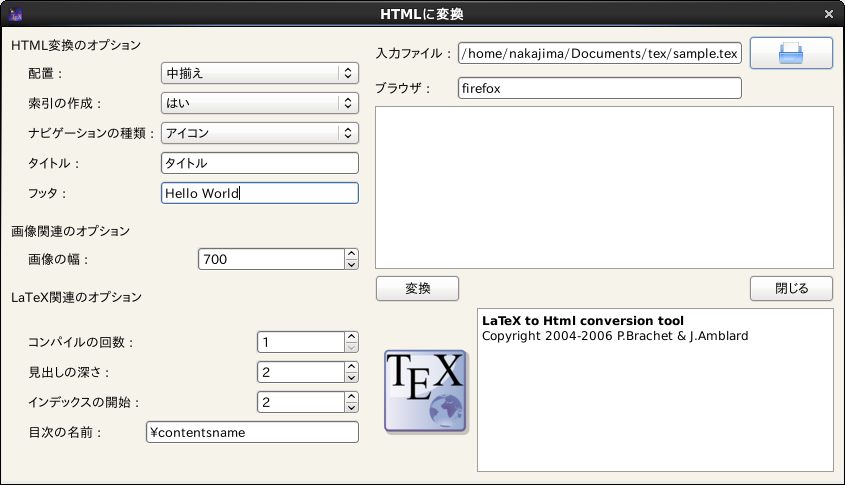
\includegraphics{doc18.png}
\caption{「HTMLへ変換」ダイアログ}
\end{figure}

\begin{figure}[htbp]
\centering
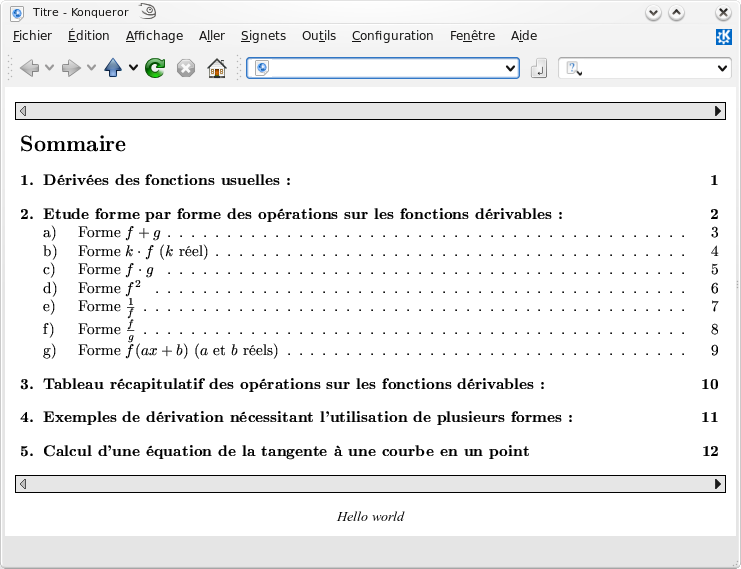
\includegraphics{doc19.png}
\caption{変換されたhtml}
\end{figure}

\section{4.9 TeXstudioでの「順方向/逆方向検索」}

\subsection{統合されたPDFビューワー}

TeXstudioでは順方向・逆方向検索を提供する統合されたPDFビューワーが提供されている。
pdflatexコマンド(または類似コマンド)でsynctexが有効化されていることを確認すること(オプション``-synctex=1''を追加する必要がある)。
もし正しく設定されていない場合、TeXstudioはコマンド自体を修正するかどうかを尋ねる。\\
順方向検索はPDFビューワーが開いた時にはいつも自動的に行われる。
TeXstudioはカーソルが現在位置している場所へ(PDF上で)移動する。
さらに、テキストエディタ上の単語をCTRL+左クリックすることでPDFへ移動したり、コンテキストメニューを用いて「PDFへ移動」を選択して移動することもできる。\\
逆方向検索は、PDF上でCTRL+左マウスボタンクリックするか、コンテキストメニュー(右マウスボタンクリック)で「ソースへ移動」を選択することで有効になる。
さらに、PDFビューワーの設定で「カーソルに続いてスクロールする」を有効化することができる。
これで、PDFビューワー上の位置をエディタ上のカーソル位置に同期させることができる。
同様に、「スクロールに続いてカーソルを移動する」を有効化することでエディタ上の位置をPDFビューワー上の位置に同期させることができる。

\subsection{外部ビューワーに対する一般的な設定}

いくつかの(dvi)ビューワーでは、(La)TeXソースファイル上のある行番号に対応するDVIファイル上での位置へ移動(あるいは視覚的に強調表示)することができる。\\
この順方向検索を有効にするには、ユーザーツール(「オプション/TeXstudioの設定」
-\textgreater{}
「ビルド」)のコマンド行または設定ダイアログのビューワーコマンド行(「オプション/TeXstudioの設定」
-\textgreater{}
「コマンド」)で、対応するビューワーのコマンドを入力すれば良い。
ビューワーが起動するときに、\textbf{@}プレースホルダは現在の行番号で置換され、\textbf{?c:ame}は現在のファイルの完全な絶対パスでのファイル名で置換される。\\\\
Windowsでは、次の形のコマンドを挿入することでDDEコマンドを実行できる:dde://service/control/{[}commands\ldots{}{]}
あるいは必要な場合次の形のコマンドでプログラムを起動することもできる(TeXstudio
1.9.9から):dde://programpath:service/control/{[}commands\ldots{}{]}\\\\
下にいくつかの一般的なビューワーに対するコマンドのリストを載せている。
当然、コマンドを使用したい場合\emph{(your program
path)}をコンピュータ上のそのプログラムのパスで置換する必要がある。\\

\subsection{Sumatra}

SumatraをTeXstudioから起動して逆方向検索を設定: "\emph{(your sumatra
path)}" -reuse-instance -inverse-search ``''``''\emph{(your TeXstudio
path)}``''" ``''``\%\%f''``'' -line \%\%l" ``?am.pdf''\\\\
起動しているSumatraである行へ移動(Windows限定):
dde://SUMATRA/control/{[}ForwardSearch(``?am.pdf'',``?c:am.tex'',@,0,0,1){]}\\\\
起動していなければSumatraを実行して、ある行へ移動(Windows限定):
dde://\emph{(your sumatra
path)}:SUMATRA/control/{[}ForwardSearch(``?am.pdf'',``?c:am.tex'',@,0,0,1){]}\\\\
SumatraからTeXstudioを実行: "\emph{(your TeXstudio path)}" ``\%f'' -line
\%l \\\\ \emph{(your Sumatra path)}の考えられる値はC:/Program
Files/SumatraPDF/SumatraPDF.exeである。

\subsection{Foxit Reader}

Foxit ReaderをTeXstudioから起動: "\emph{(your Reader path)"} ``?am.pdf''

\subsection{Acrobat Reader}

TeXstudioからAcrobat Readerを起動: "\emph{(your Reader path)"}
``?am.pdf''\\\\ 実行しているAcrobat
Reader上のある位置へ移動(Windows限定):
dde://acroview/control/{[}DocOpen(``?am.pdf''){]}{[}FileOpen(``?am.pdf''){]}{[}DocGotoNameDest(``?am.pdf'',``jump-position''){]}
~~ ~~ ~~\emph{jump-positionはhyperrefパッケージで定義できる}\\\\
実行しているAcrobat Reader上の文書を閉じる(Windows限定):
dde://acroview/control/{[}DocOpen(``?am.pdf''){]}{[}FileOpen(``?am.pdf''){]}{[}DocClose(``?am.pdf''){]}

\subsection{Yap (Yet Another Previewer)}

TeXstudioからYapを起動: "\emph{(your Yap path)}" -1 -s @?c:m.tex \%.dvi
\\\\ YapからTeXstudioを起動: "\emph{(your TeXstudio path)}" ``\%f''
-line \%l \\\\ \emph{(your Yap path)}の考えられる値はC:/Program
Files/MiKTeX 2.7/miktex/bin/yap.exeである。

\subsection{xdvi}

TeXstudioからxdviを起動: xdvi \%.dvi -sourceposition @:?c:m.tex\\\\
TeXstudioからxdviを起動して逆方向検索を有効化: xdvi -editor ``texstudio
\%f -line'' \%.dvi -sourceposition @:\%.tex

\subsection{kdvi}

TeXstudioからkdviを起動: kdvi ``file:\%.dvi\#src:@ ?c:m.tex''

\subsection{Okular}

TeXstudioからokularを起動: okular --unique \%.dvi\#src:@?c:m.tex\\\\
OkularからTeXstudioを起動: texstudio \%f -line \%l

\subsection{Skim}

TeXstudioからSkimを起動: (your Skim
path)/Contents/SharedSupport/displayline @ ?am.pdf ?c:ame\\\\
SkimからTeXstudioを起動:
コマンド:/applications/texstudio.app/contents/macos/texstudio
引数:``\%file'' -line \%line \\\\ \emph{(your Skim
path)}の考えられる値は/Applications/Skim.appである。

\section{4.10 高度なヘッダの使用法}

Texstudioでは、テキストに特殊な「マジック」コメントを配置して、その文書にあるオプションを適応させることができる。

\begin{itemize}
\item
  \lstinline"% !TeX spellcheck = de_DE"

  この特殊コメントはTXSに、文書がドイツ語で書かれていて一般的な設定とは別にドイツ語のスペルチェックを用いることを教えている。
\item
  \lstinline"% !TeX encoding = utf8"

  このコードは文書の文字エンコーディングを定義している。
\item
  \lstinline"% !TeX root = filename"

  このコードはこのファイルに対するマスターファイルを定義している。
\item
  \lstinline"% !TeX program = pdflatex"

  このコードは文書がpdflatexでコンパイルされることを明示している(つまり既定のtxs:///quickコマンドを上書きする)。
\item
  \lstinline"% !TeX TXS-program:latex = txs:///xelatex %"

  このコードは既定のtxs:///latexコマンドを上書きして代わりにxelatexを呼び出す。
\item
  \lstinline# % !TeX TXS-SCRIPT = foobar % //Trigger = ?load-this-file % app.load("/tmp/test/test.tex"); % app.load("/tmp/test/a.tex"); % TXS-SCRIPT-END     #

  このコードは一時的なjavascriptマクロを定義している。
  このマクロはファイルが読み込まれた時に実行され、順番に/tmp/testにある2つのファイルを読み込む。
\end{itemize}

\section{4.11 TeXstudioコマンドの概要}

\lstinline!texstudio file [--master] [--line xx[:cc]] [--insert-cite citation] [--start-always] [--pdf-viewer-only] [--page yy]!\\\\

\lstinline!--master!

文書をマスターファイルとして定義

\lstinline!--line xx[:cc]!

TeXstudioは文書読み込み後にxx行へ移動する。
さらにコロンで区切って目標の列を追加できる(例:``--line
2:5''は2行目の5列目に移動する)。

\lstinline!--insert-cite citation!

カーソル位置へ挿入するbibtexキーをTeXstudioへ通知する。
これは外部参考文献管理アプリケーションに対するインターフェースとして、引用をTeXstudioに通知するために用いられる。
\textbackslash{}mycite\{key\}のようなコマンド(カスタマイズされていても良い)または、キーだけを渡してもよい。
後者の場合、\textbackslash{}cite\{key\}に展開される。
また、カンマ区切りのキーリストもサポートされている。
カーソルがすでに引用マクロ内にある場合、TeXstudioはそれを認識する。
その場合キーのみが適切な位置に挿入され、そうでない場合完全な引用コマンドが挿入される。

\lstinline!--start-always!

TeXstudioの別のインスタンスがすでに起動していても、TeXstudioを起動する。
これで複数のインスタンスを利用できる。

\lstinline!--pdf-viewer-only!

TeXstudioを、エディタなしの単体のPDFビューワーとして開く。

\lstinline!--page!

オプションであり、PDFビューワーとして用いた場合にTeXstudioで特定のページを表示する。

次の追加のオプションはTeXstudioのデバッグ版でのみ利用できる:

\ctable[pos = H, center, botcap]{ll}
{% notes
}
{% rows
\FL
\lstinline!--disable-tests! & あらゆるテストを実行しない。
\\\noalign{\medskip}
\lstinline!--execute-tests! & 最も一般的なテストを強制的に実行する。
\\\noalign{\medskip}
\lstinline!--execute-all-tests! & 全てのテストを強制的に実行する。
\LL
}

注:実行ファイルに変更がある場合(つまり、TXSが最後の実行以来コンパイルされてきた)、最も一般的なテストは自動的に実行される。
さらに全てのテストは週一で実行される。

\section{4.12 キーボードショートカット}

既定のキーボードショートカット:

\begin{itemize}
\item
  「ファイル」メニュー:

  \begin{itemize}
  \item
    新規作成:Ctrl+N
  \item
    開く:Ctrl+O
  \item
    保存:Ctrl+S
  \item
    名前をつけて保存:Ctrl+Alt+S
  \item
    全て保存:Ctrl+Shift+Alt+S
  \item
    閉じる:Ctrl+W
  \item
    印刷:Ctrl+P
  \item
    終了:Ctrl+Q
  \end{itemize}
\item
  「編集」メニュー:

  \begin{itemize}
  \item
    元に戻す:Ctrl+Z
  \item
    やり直す:Ctrl+Y
  \item
    コピー:Ctrl+C
  \item
    切り取り:Ctrl+X
  \item
    貼り付け:Ctrl+V
  \item
    LaTeXとして貼り付け:Ctrl+Shift+V(「Idefix」メニュー)
  \item
    全て選択:Ctrl+A
  \item
    行を削除:Ctrl+K
  \item
    プレビューの表示:Alt+P(「Idefix」メニュー)
  \item
    検索:Ctrl+F
  \item
    検索を続ける:Ctrl+M
  \item
    置換:Ctrl+R
  \item
    特定の行番号へ移動:Ctrl+G
  \item
    前の変更へ移動:Ctrl+H
  \item
    次の変更へ移動:Ctrl+Shift+H
  \item
    ブックマーク0..9の切り替え:Ctrl+Shift+0..9
  \item
    ブックマーク0..9へ移動:Ctrl+0..9
  \item
    次のマークへ移動:Ctrl+Down
  \item
    前のマークへ移動:Ctrl+Up
  \item
    次のLaTeXエラーへ移動:Ctrl+Shift+Down(「Idefix」メニュー)
  \item
    前のLaTeXエラーへ移動:Ctrl+Shift+Up(「Idefix」メニュー)
  \item
    次のLaTeXの良くないボックスへ移動:Shift+Alt+Down(「Idefix」メニュー)
  \item
    前のLaTeXの良くないボックスへ移動:Shift+Alt+Up(「Idefix」メニュー)
  \item
    定義へ移動:Ctrl+Alt+F(「Idefix」メニュー)
  \item
    プレースホルダーを削除:Ctrl+Shift+K(「Idefix」メニュー)
  \end{itemize}
\item
  「ツール」メニュー:

  \begin{itemize}
  \item
    ビルド&表示:F1
  \item
    コンパイル:F6
  \item
    表示:F7
  \item
    文献(Bibtex):F11
  \item
    索引生成:F12
  \item
    (カーソル位置から)スペルチェック:Ctrl+Shift+F7
  \item
    類語辞典を開く:Ctrl+Shift+F8
  \end{itemize}
\item
  「LaTeX」メニュー:

  \begin{itemize}
  \item
    箇条書きの項目(\textbackslash{}item):Ctrl+Shift+I
  \item
    イタリック体:Ctrl+I
  \item
    スラント体:Ctrl+Shift+S
  \item
    ボールド体:Ctrl+B
  \item
    タイプライター体:Ctrl+Shift+T
  \item
    スモールキャップス体:Ctrl+Shift+C
  \item
    強調:Ctrl+Shift+E
  \item
    強制改行:Ctrl+Return
  \item
    begin\{environment\}:Ctrl+E
  \item
    次のラベルに参照(\textbackslash{}ref)を挿入:Ctrl+Alt+R
  \end{itemize}
\item
  「数式」メニュー:

  \begin{itemize}
  \item
    インライン数式:Ctrl+Shift+M
  \item
    ディスプレイ数式:Alt+Shift+M
  \item
    番号付き数式:Ctrl+Shift+N
  \item
    下付き添字:Ctrl+Shift+D
  \item
    上付き添字:Ctrl+Shift+U
  \item
    \textbackslash{}frac:Alt+Shift+F
  \item
    \textbackslash{}dfrac:Ctrl+Shift+F
  \item
    \textbackslash{}sqrt:Ctrl+Shift+Q
  \item
    \textbackslash{}left:Ctrl+Shift+L
  \item
    \textbackslash{}right:Ctrl+Shift+R
  \end{itemize}
\item
  「表示」メニュー:

  \begin{itemize}
  \item
    前の文書:Ctrl+PgUp
  \item
    次の文書:Ctrl+PgDown
  \end{itemize}
\end{itemize}

\section{4.13 cwl形式の解説}

cwlファイルは、考えられるコマンドの提案のため補完の際に用いられたり、入力したコマンドが実存しているかどうか確認するための構文チェックの際に用いられたりする。
cwlファイルの各行ではコマンドが定義されている。
コメント行も可能であり、\lstinline!#!で始めればよい。
コマンド構文は次の形で表される。

\lstinline!<command>[#classification]!\\

分類classificationがない場合、そのコマンドはLaTeX文書のあらゆる位置で有効であるとみなされる。
文字\lstinline!#!は、次のような特別な意味があるので、\lstinline!command!内で使用することはできない:

\begin{itemize}
\item
  \# (行の開始時):コメント
\item
  \# (後ろで):コマンド分類に対する区切り記号
\end{itemize}

\subsection{4.13.1 コマンド書式}

コマンドは、文書中に見られるような単なる有効なLaTeX表現である(例:\lstinline!\section{title}!)。
改行を\lstinline!%n!でコマンド内に含めることもできる。
既定では、全てのオプションはプレースホルダとして扱われる。
その代わりに、\lstinline!%|!でカーソルの停止位置を定義する(例:\lstinline!\left(%|\right)!)か、\lstinline!%< %>!を用いてオプションの一部のみをプレースホルダとしてしるし付けしてもよい(例:\lstinline!\includegraphics[scale=%<1%>]{file}!)。

\subsection{4.13.2 分類の書式}

次の分類がTXSでは有効である:

分類子

意味

*

「全て」タブでのみ補完に用いられる珍しいコマンド。
この印は他の分類子とともに用いてもよい。

S

補完の際に全く表示されない。 この印は他の分類子とともに用いてもよい。

m

数式環境でのみ有効

t

tabular環境(または同様の環境)でのみ有効

T

tabbing環境でのみ有効

n

テキスト環境(つまり数式環境でない)でのみ有効

r

このコマンドは``\textbackslash{}ref\{key\}''のような参照を表すことを示す。

c

このコマンドは``\textbackslash{}cite\{key\}''のような引用を表すことを示す。

l

このコマンドは``\textbackslash{}label\{key\}''のようなラベルを表すことを示す。

d

このコマンドは``\textbackslash{}newcommand\{cmd\}\{def\}''のような定義コマンドを表すことを示す。

g

このコマンドは``\textbackslash{}includegraphics\{file\}''のような画像読み込みコマンドを表すことを示す。

i

このコマンドは``\textbackslash{}include\{file\}''のようなファイル読み込みコマンドを表すことを示す。

u

このコマンドは``\textbackslash{}usepackage\{package\}''のようなパッケージ使用コマンドを表すことを示す。

b

このコマンドは``\textbackslash{}bibliography\{bib\}''のような参考文献を表すことを示す。

U

このコマンドは``\textbackslash{}url\{URL\}''のようなurlコマンドを表すことを示す(ただしURLはチェックされない)

/env1,env2,\ldots{}

環境env1、env2\ldots{}内でのみ有効

\textbackslash{}env

環境の別名であることを表し、``env''環境のようにその環境が扱われることを意味する。
これはenv=math, tabularに対して有用である。

例:\\

行

解説

\lstinline!# test!

コメント

\lstinline!\typein{msg}#*!

「全て」タブの補完にのみ表示される珍しいコマンド

\lstinline!\sqrt{arg}#m!

数式モードでのみ有効

\lstinline!\pageref{key}#r!

補完に正しく使用される参照コマンドを表す。

\lstinline!\vector(xslope,yslope){length}#*/picture!

picture環境でのみ有効な珍しいコマンド

\lstinline!\begin{align}#\math!

コマンドの妥当性や構文強調に関しては、``align''環境が数式環境のように扱われることを表す!

\section{4.14 表テンプレートの使用}

Texstudioでは、表テンプレートに従って既存のLaTeX形式の表を書式変更できるようにしている。\\
例えば、TXSで次の表を入力したとする:

\begin{lstlisting}
\begin{tabular}{ll}
a&b\\
c&d\\
\end{tabular}
\end{lstlisting}

カーソルをその表の内部に置き、メニュー「LaTeX/表の操作/テンプレートを用いて表を再構築する」を選択する。\\
すると表の書式を定義するテンプレートを選択することができる。
多数のテンプレートがTXSで予め定義されている:

\begin{itemize}
\item
  fullyframed\_firstBold
\item
  fullyframed\_longtable
\item
  plain\_tabular
\item
  plain\_tabularx
\item
  rowcolors\_tabular
\end{itemize}

最初の項目を選択すると、表は次のように書式変更される:

\begin{lstlisting}
\begin{tabular}{|l|l|}
\hline
\textbf{a}&\textbf{b}\\ \hline
c&d\\ \hline
\end{tabular}
\end{lstlisting}

これらのテンプレートで予め定義された様式にちなんで容易に表を書式変更できるようになる。
従って、文書中の表が非常に単純な形式で入力されている場合でもその表の形式を同一のものにすることができる。

\subsection{4.14.1 表テンプレートの作成}

テンプレートはユーザーが定義することもできる。
テンプレートは設定ディレクトリ(Linux:
\textasciitilde{}/.config/texstudio)に置いて、設定tabletemplate\_\emph{name}.jsにちなんで名前をつける必要がある。

メタデータを用いてテンプレートの追加の情報を提供できる。
メタデータはソースコードの\lstinline!metaData!に保存される。
コード\lstinline!var metaData = {!はファイルの最初の行で始めなければならない。
現在文字列値のみが利用できる。
また、整形にhtmlタグを使用することができる。 例:

\begin{lstlisting}
var metaData = {
"Name"       : "Colored rows",
"Description" : "Formats the table using alternate colors for rows. <br> <code>\usepackage[table]{xcolor}</code> is necessary.", 
"Author"      : "Jan Sundermeyer",
"Date"        : "4.9.2011",
"Version"     : "1.0"
}
\end{lstlisting}

テンプレート自体は、表全体を含むいくつかの予め定義された変数を持つjavascript(上記参照)である。
新しい表は古いものの置換として配置されるだけであり、その変数から情報を使用する。
4つの変数が与えられている:

\begin{itemize}
\item
  def
  あらゆる書式なしの単純な表定義(つまり、\textbar{}l\textbar{}l\textbar{}の代わりにllを使用)
\item
  defSplit 列で分割された表定義(配列array=l,l,p\{2cm\})
\item
  env ``tabular''や``longtable''のような古い表の実際の環境名
\item
  tab 実際の表。
  これは行のリストであり、各行はセルの内容を文字列として含む列のリストである。
\end{itemize}

\\

行われることの本質を見るために、``plain\_tabular''テンプレートのソースをここに載せておく。

\begin{lstlisting}
function print(str){ //ソースをより見やすくするためこの関数を定義
cursor.insertText(str)
}
function println(str){ //ソースをより見やすくするためこの関数を定義
cursor.insertText(str+"\n")
}
println("\\begin{tabular}{"+defSplit.join("")+"}") //表環境を出力
for(var i=0;i<tab.length;i++){  //表の全ての行に対してループ
    var line=tab[i];  //lineは行row[i]の全ての列のリスト
    for(var j=0;j<line.length;j++){ //行の全ての列に対してループ
        print(line[j]) //セルを出力
        if(j<line.length-1) //最後の列で無い場合
            print("&") //&を出力
    }
    println("\\\\") // \\で行を終える。文字列中にバックスラッシュが必要なことに注意。
}
println("\\end{tabular}") //環境を閉じる
\end{lstlisting}

例で見たように、表は完全に再構築される必要があり、それから新しい書式が適用可能となる。
2番めの例は幾分手の込んだ表を出力する(fullyframed\_firstBold):

\begin{lstlisting}
function print(str){
cursor.insertText(str)
}
function println(str){
cursor.insertText(str+"\n")
}
if(env=="tabularx"){
  println("\\begin{tabularx}{\\linewidth}{|"+defSplit.join("|")+"|}")
}else{
    println("\\begin{"+env+"}{|"+defSplit.join("|")+"|}")
}
println("\\hline")
for(var i=0;i<tab.length;i++){
    var line=tab[i];
    for(var j=0;j<line.length;j++){
                var col=line[j];
                var mt=col.match(/^\\textbf/);
                if(i==0 && !mt)
                  print("\\textbf{")
        print(line[j])
                if(i==0 && !mt)
                  print("}")
        if(j<line.length-1)
            print("&")
    }
    println("\\\\ \\hline")
}
println("\\end{"+env+"}")
\end{lstlisting}

\end{document}
